\documentclass[a4paper, 12pt]{book}
\usepackage[italian]{babel}

\usepackage[]{csvsimple}
\usepackage{float}

\usepackage{ragged2e}
\usepackage[left=25mm, right=25mm, top=15mm]{geometry}
\geometry{a4paper}
\usepackage{graphicx}
\usepackage{booktabs}
\usepackage{paralist}
\usepackage{subfig} 
\usepackage{fancyhdr}
\usepackage{amsmath}
\usepackage{amssymb}
\usepackage{amsfonts}
\usepackage{amsthm}
\usepackage{mathtools}
\usepackage{enumitem}
\usepackage{titlesec}
\usepackage{braket}
\usepackage{gensymb}
\usepackage{url}
\usepackage{hyperref}
\usepackage{csquotes}
\usepackage{multicol}
\usepackage{graphicx}
\usepackage{wrapfig}
\usepackage{caption}

\usepackage{esint}

\captionsetup{font=small}
\pagestyle{fancy}
\renewcommand{\headrulewidth}{0pt}
\lhead{}\chead{}\rhead{}
\lfoot{}\cfoot{\thepage}\rfoot{}
\usepackage{sectsty}
\usepackage[nottoc,notlof,notlot]{tocbibind}
\usepackage[titles,subfigure]{tocloft}
\renewcommand{\cftsecfont}{\rmfamily\mdseries\upshape}
\renewcommand{\cftsecpagefont}{\rmfamily\mdseries\upshape}

\let\oldsection\section% Store \section
\renewcommand{\section}{% Update \section
	\renewcommand{\theequation}{\thesection.\arabic{equation}}% Update equation number
	\oldsection}% Regular \section
\let\oldsubsection\subsection% Store \subsection
\renewcommand{\subsection}{% Update \subsection
	\renewcommand{\theequation}{\thesubsection.\arabic{equation}}% Update equation number
	\oldsubsection}% Regular \subsection

\newcommand{\abs}[1]{\left\lvert#1\right\rvert}
\newcommand{\norm}[1]{\left\lVert#1\right\rVert}
\newcommand{\vprod}[2]{\vec{#1}\times\vec{#2}}
\newcommand{\sprod}[2]{\vec{#1}\cdot\vec{#2}}

\newcommand{\g}{\text{g}}
\newcommand{\m}{\text{m}}
\newcommand{\cm}{\text{cm}}
\newcommand{\mm}{\text{mm}}
\newcommand{\s}{\text{s}}
\newcommand{\N}{\text{N}}
\newcommand{\Hz}{\text{Hz}}

\newcommand{\virgolette}[1]{``\text{#1}"}
\newcommand{\tildetext}{\raise.17ex\hbox{$\scriptstyle\mathtt{\sim}$}}

\renewcommand{\arraystretch}{1.2}

\addto\captionsenglish{\renewcommand{\figurename}{Fig.}}
\addto\captionsenglish{\renewcommand{\tablename}{Tab.}}

\DeclareCaptionLabelFormat{andtable}{#1~#2  \&  \tablename~\thetable}

\setlength{\parindent}{0pt}

\newcommand{\dive}{\nabla\cdot}
\newcommand{\rot}{\nabla\times}

\graphicspath{{./images/}}

\title{\Huge\textbf{Struttura della Materia} \\ \large Prof. G. Onida a.a. 2024-25}
\author{Leonardo Cerasi%
	\thanks{\scriptsize\href{mailto:leonardo.cerasi@studenti.unimi.it}{leo.cerasi@pm.me}}%
	, Lucrezia Bioni\\
	\small GitHub repository: \href{https://github.com/LeonardoCerasi/notes}{LeonardoCerasi/notes}}

\begin{document}

\frontmatter

\maketitle
\tableofcontents
\pagestyle{indice}

\mainmatter

\chapter*{Introduzione}
\pagestyle{introd}
\addcontentsline{toc}{chapter}{Introduzione}
\markboth{Introduzione}{}
\selectlanguage{italian}

Il problema generale che si va ad analizzare è il sistema di $ N_n $ elettroni ed $ N_n $ nuclei atomici, il cui moto non-relativistico è affetto solo dall'interazione elettromagnetica ed è dunque descritto dall'Hamiltoniana:
\begin{equation*}
	\mathcal{H} = T_n + T_e + V_{ne} + V_{nn} + V_{ee}
\end{equation*}
L'energia cinetica totale dei nuclei è:
\begin{equation*}
	T_n = \frac{1}{2} \sum_\alpha \frac{\ve{P}_{\ve{R}_\alpha}^2}{M_\alpha}
\end{equation*}
dove $ \ve{P}_{\ve{R}_\alpha} $ è il momento coniugato alla posizione $ \ve{R}_\alpha $ dell'$ \alpha $-esimo nucleo, mentre l'energia cinetica degli elettroni è:
\begin{equation*}
	T_e = \frac{1}{2m_e} \sum_i \ve{P}_{\ve{r}_i}^2
\end{equation*}
dove $ \ve{P}_{\ve{r}_i} $ è il momento coniugato alla posizione $ \ve{r}_i $ dell'$ i $-esimo elettrone. I potenziali d'interazione elettromagnetica sono invece:
\begin{equation*}
	V_{ne} = - \frac{q_e^2}{4\pi \epsilon_0} \sum_\alpha \sum_i \frac{Z_\alpha}{\abs{\ve{R}_\alpha - \ve{r}_i}}
\end{equation*}
\begin{equation*}
	V_{nn} = \frac{q_e^2}{4\pi \epsilon_0} \frac{1}{2} \sum_\alpha \sum_{\beta \neq \alpha} \frac{Z_\alpha Z_\beta}{\abs{\ve{r}_\alpha - \ve{r}_\beta}}
\end{equation*}
\begin{equation*}
	V_{ee} = \frac{q_e^2}{4\pi \epsilon_0} \frac{1}{2} \sum_i \sum_{j \neq i} \frac{1}{\abs{\ve{r}_i - \ve{r}_j}}
\end{equation*}
La risoluzione analitica di questo problema è possibile solo in un numero limitato di casi, mentre la sua integrazione numerica scala in complessità esponenzialmente con $ N = N_e + N_n $.\\
Nella formulazione di tale Hamiltoniana, si sono applicate alcune approssimazioni:
\begin{enumerate}
	\item corpi puntiformi: mentre per l'elettrone, in quanto particella fondamentale, questa assunzione è sempre lecita, per il nucleo atomico essa è possibile visto che il rapporto tra raggio nucleare e raggio atomico è dell'ordine di $ 10^{-3} $, oltre al fatto che le energie in gioco nei processi atomici ($ \sim 1\ev $) non sono sufficienti ad eccitare i gradi di libertà interni del nucleo ($ \sim 1\mev $);
	\item moto non-relativistico: alcune correzioni relativistiche (es.: interazione spin-orbita) possono essere trattate perturbativamente;
	\item sistema isolato: si assume il sistema non-interagente con l'ambiente esterno ed in assenza di campi esterni.
\end{enumerate}
Si noti che mentre i sistemi a singola particella godono di determinate simmetrie, quelli a molti corpi possono presentare delle rotture spontanee di simmetria: ciò è particolarmente evidente nei sistemi molecolari, mentre in quelli atomici è presente ma in misura minore, ed avviene poiché nei casi in cui una rottura di simmetria permetta di abbassare l'energia totale del sistema.

\paragraph{Ordini di grandezza}

Innanzitutto, conviene definire la coupling constant dell'interazione elettromagnetica:
\begin{equation*}
	e^2 \equiv \frac{q_e^2}{4\pi \epsilon_0} = 2.3071 \cdot 10^{-28} \,\text{J} \,\text{m} = 14.3387 \ev \ang
\end{equation*}
La scala del moto elettronico nell'atomo è data dal \textit{raggio di Bohr}:
\begin{equation*}
	a_0 \equiv \frac{\hbar^2}{m_e e^2} = 0.529177 \cdot 10^{-10} \,\text{m} = 0.529177 \ang
\end{equation*}
Evidenze sperimentali mostrano che gli atomi nella materia sono distanziati nell'ordine di $ 2a_0 - 10a_0 $. La scala delle interazioni elettromagnetiche in ambito atomico/molecolare è dunque data dall'\textit{energia di Hartree}:
\begin{equation*}
	E_\text{Ha} \equiv \frac{e^2}{a_0} = 4.35974 \cdot 10^{-18} \,\text{J} = 27.2114 \ev
\end{equation*}
La tipica timescale del moto elettronico si ottiene dal principio d'indeterminazione:
\begin{equation*}
	t_0 = \frac{\hbar}{E_\text{Ha}} = 2.4189 \cdot 10^{-17} \,\text{s}
\end{equation*}
Ciò permette di calcolare la scala delle velocità elettroniche, confermando l'approssimazione non-relativistica:
\begin{equation*}
	v_0 = \frac{a_0}{t_0} = 2.1877 \cdot 10^6 \,\text{m} \,\text{s}^{-1} \simeq 0.01 c
\end{equation*}
La scala dei fenomeni relativistici nella dinamica elettronica è data dalla \textit{costante di struttura fine}:
\begin{equation*}
	\alpha = \frac{v_0}{c} = \frac{e^2}{\hbar c} = 7.29734 \cdot 10^{-3} \simeq \frac{1}{137.036}
\end{equation*}
Comparando con le onde elettromagnetiche, la scala delle distanze interatomiche ($ \sim 1\ang $) corrisponde alla regione dei raggi X, mentre quella delle frequenze elettroniche (e dunque di $ E_\text{Ha} $) corrisponde alla fascia UV ($ \lambda \sim 10^3 a_0 $); le frequenze tipiche (e dunque le energie) del moto nucleare sono invece associate alla regione IR ($ \nu \sim 5 \,\text{THz} $).

\paragraph{Spettroscopia}

Gli esperimenti spettroscopici sono quelli in cui una proprietà caratterizzante l'interazione tra radiazione e materia è misurata in funzione della frequenza della radiazione incidente sul campione che si vuole studiare. I principali tipi di spettroscopia sono due:
\begin{enumerate}
	\item assorbimento: un fascio collimato di luce monocromatica incide sul bersaglio; se la frequenza della radiazione coincide con quella di una transizione specifica del campione, ci sarà un importante assorbimento di fotoni: questo sarà visibile plottando l'intensità della radiazione emergente dal campione $ I(\omega) $, ottenendo il cosiddetto spettro d'assorbimento;
	\item emissione: il campione viene portato in uno stato eccitato (es.: bombardandolo di elettroni o fotoni alto-energetici), dunque emetterà della radiazione ad ogni transizione di diseccitamento, la quale va a formare il cosiddetto spettro d'emissione.
\end{enumerate}
Gli spettri atomici e molecolari sono dunque caratterizzati da picchi monocromatici, detti linee, associate a transizioni risonanti tra stati $ \ket{i} , \ket{f} $ che determinano linee a $ \omega_{if} = \frac{1}{\hbar} \abs{E_i - E_f} $. Sebbene a livello teorico queste linee sarebbero delle $ \delta $ di Dirac, sperimentalmente si misurano sempre delle righe più o meno strette; le cause dell'allargamento delle linee spettrali sono sia intrinseche che estrinseche, e principalmente sono:
\begin{enumerate}
	\item risoluzione sperimentale: tipicamente determinata da vari effetti aleatori, dunque determina una forma gaussiana; può essere migliorata con accorgimenti tecnici;
	\item allargamento naturale: dovuto al fatto che gli stati eccitati, sebbene stazionari in prima approssimazione, vengono resi instabili dall'interazione col le fluttuazioni di punto-zero del campo elettromagnetico (quantistico); si determina dunque un decadimento spontaneo di tutti gli autostati d'energia (eccetto il ground state) che, sebbene randomico per un singolo atomo, segue una legge statistica per un sistema a molti atomi:
	\begin{equation*}
		N(t) = N_0 e^{- \gamma t} = N_0 e^{- t / \tau}
	\end{equation*}
	dove $ \gamma $ è la costante di decadimento e $ \tau $ la vita media dello stato eccitato, la quale setta la durata tipica della spettroscopia. Dal principio d'indeterminazione, si trova che l'energia di uno stato eccitato non è misurabile con precisione migliore di:
	\begin{equation*}
		\Delta E = \frac{\hbar}{\tau} = \hbar \gamma
	\end{equation*}
	Ciò causa dunque l'allargamento naturale delle linee spettrali secondo la Lorentziana:
	\begin{equation*}
		I(\omega) = I_0 \frac{\gamma^2}{(\omega - \omega_{if})^2 + \gamma^2}
	\end{equation*}
	Gli stati atomici eccitati hanno $ \tau \sim 1\,\text{ns} $, dunque l'allargamento è di $ \Delta E \sim 1\,\mu\text{eV} $.
	\item allargamento Doppler: nel caso di un campione in fase gassosa, il moto termico randomico degli atomi/molecole determina un red/blue-shift delle frequenze di transizione, a seconda della velocità casuale dell'atomo/molecola che decade; si ha un allargamento gaussiano delle righe spettrali, che determina:
	\begin{equation*}
		\Delta \omega_\text{Doppler} = \omega_{if} \sqrt{8 \ln(2) \frac{k_B T}{M c^2}}
	\end{equation*}
	A temperatura fissata, gli atomi/molecole più leggeri si muoveranno più velocemente, determinando un allargamento maggiore (sempre nell'ordine dei $ \mu\text{eV} $).
\end{enumerate}
Si ha dunque un allargamento totale pari alla somma in quadratura di questi allargamenti singoli.












\part{Atomi}
\pagestyle{body}

\chapter{Atomi Idrogenoidi}
\selectlanguage{italian}

\section{Principio variazionale di Ritz}

Per lo studio di un sistema quantistico, è utile dimostrare un principio variazionale sul valore di aspettazione dell'Hamiltoniana $ \mathcal{H} $ del sistema, ovvero sull'energia:
\begin{equation}
	E[\psi] \defeq \frac{\braket{\psi | \mathcal{H} | \psi}}{\braket{\psi | \psi}} \in \R
\end{equation}

\begin{proposition}{}{}
	Il valore di aspettazione di una Hamiltoniana su un suo autostato è stazionario.

	\tcblower

	\begin{proof}
		Prendendo una variazione infinitesima $ \ket{\psi + \delta\psi} $ ed usando $ \mathcal{H} \ket{\psi} = E[\psi] \ket{\psi} $:
		\begin{equation*}
			\begin{split}
				\delta E
				&= E[\psi + \delta\psi] - E[\psi] = \frac{\braket{\psi + \delta\psi | \mathcal{H} | \psi + \delta\psi}}{\braket{\psi + \delta\psi | \psi + \delta\psi}} - \frac{\braket{\psi | \mathcal{H} | \psi}}{\braket{\psi | \psi}} \\
				&\simeq \frac{\braket{\psi | \mathcal{H} | \psi} + \braket{\psi | \mathcal{H} | \delta\psi} + \braket{\delta\psi | \mathcal{H} | \psi}}{\braket{\psi | \psi} + \braket{\psi | \delta\psi} + \braket{\delta\psi | \psi}} - \frac{\braket{\psi | \mathcal{H} | \psi}}{\braket{\psi | \psi}} \\
				&= \frac{\braket{\psi | \mathcal{H} | \delta\psi} + \braket{\delta\psi | \mathcal{H} | \psi} - E[\psi] \braket{\psi | \delta\psi} - E[\psi] \braket{\delta\psi | \psi}}{\braket{\psi | \psi} + \braket{\psi | \delta\psi} + \braket{\delta\psi | \psi}} \\
				&= \frac{2\Re \braket{\delta\psi | (\mathcal{H} - E[\psi]) | \psi}}{\braket{\psi | \psi} + \braket{\psi | \delta\psi} + \braket{\delta\psi | \psi}} = 0
			\end{split}
		\end{equation*}
	\end{proof}
\end{proposition}

\begin{theorem}{Principio variazionale di Ritz}{}
	Detto $ \ket{\psi_0} $ lo stato fondamentale di $ \mathcal{H} $, allora $ E[\psi] \ge E[\psi_0] \equiv E_0 \,\,\forall \ket{\psi} \in \mathscr{H} $.

	\tcblower
	\begin{proof}
		Data una base di autostati $ \{u_n\} : \mathcal{H} \ket{u_n} = E_n \ket{u_n} \land \braket{u_n | u_m} = \delta_{nm} $, dove $ u_0 $ è il ground state con $ E_0 \le E_1 \le E_2 \le \dots $, per il generico stato $ \ket{\psi} = \sum_n A_n \ket{u_n} $:
		\begin{equation*}
			E[\psi] - E_0
			= \frac{\abs{A_0}^2 E_0 + \sum_{i \neq 0} \abs{A_i}^2 E_i}{\abs{A_0}^2 + \sum_{i \neq 0} \abs{A_i}^2} - E_0 = \frac{\sum_{i \neq 0} \left( E_i - E_0 \right) \abs{A_i}^2}{\abs{A_0}^2 + \sum_{i \neq 0} \abs{A_i}^2} \ge 0
		\end{equation*}
	\end{proof}
\end{theorem}

Questo risultato è utile poiché permette di trovare il ground state minimizzando l'energia: se si parametrizza la funzione d'onda, il ground state sarà dato dal set di parametri per cui si ha il minimo dell'energia.\\
Una possibile applicazione è quella di ottimizzare i coefficienti di uno sviluppo di una funzione d'onda su una base di funzioni d'onda fissate: vedendo i coefficienti della combinazione lineare come parametri, minimizzando l'energia si ottiene un sistema lineare di equazioni la cui risoluzione fornisce i parametri che meglio approssimano la funzione d'onda reale. Questo è il caso, ad esempio, della Linear Combination of Atomic Orbital, nel quale si esprime la funzione d'onda di una molecola come combinazione lineare delle funzioni d'onda dei suoi atomi costituenti.\\
Questo metodo può essere ulteriormente generalizzato facendo variare parametricamente anche le funzioni d'onda di base sulle quali si effettua lo sviluppo (es.: metodo di Hartree-Fock).

\section{Soluzione analitica}

L'atomo a singolo elettrone (o idrogenoide) è uno dei pochi casi in cui l'equazione di Schrödinger può essere risolta analiticamente. Essendo il potenziale coulombiano un potenziale radiale a simmetria sferica, si può separare il problema in moto del centro di massa e moto radiale: essendo la massa nucleo $ M $ migliaia di volte quella dell'elettrone $ m_e $, il centro di massa può essere approssimato con la posizione stessa del nucleo. La correzione di massa ridotta diventa importante quando si considerano atomi esotici, come ad esempio l'idrogeno muonico (sistema legato protone-muone).\\
Concentrandosi sull'Hamiltoniana di moto relativo (quella del centro di massa è semplicemente l'Hamiltoniana di particella libera):
\begin{equation}
	\mathcal{H} = - \frac{\hbar^2}{2\mu} \nabla_\ve{r}^2 - \frac{Ze}{r}
	\label{eq:1-e-ham}
\end{equation}
dove $ \ve{r} \equiv \ve{R} - \ve{r}_e $ e $ \mu \equiv (M^{-1} + m_e^{-1})^{-1} $. In coordinate sferiche si trova:
\begin{equation*}
	\nabla^2 = \frac{2}{r} \frac{\pa}{\pa r} + \frac{\pa^2}{\pa r^2} - \frac{\hat{L}^2}{\hbar^2 r^2}
\end{equation*}
Dato che $ [\mathcal{H} , \hat{L}^2] = 0 $, si può cercare una soluzione $ \psi = \psi(r,\vartheta,\varphi) $ in funzione delle autofunzioni di $ \hat{L}^2 $: questi sono le armoniche sferiche $ Y_{\ell,m} : \hat{L}^2 Y_{\ell,m} = \hbar^2 \ell (\ell + 1) Y_{\ell,m} $, con $ \ell \in \N_0 $ e $ -\ell \le m \le \ell $. Scrivendo $ \psi(r,\vartheta,\varphi) = R(r) Y_{\ell,m}(\vartheta,\varphi) $ si ha:
\begin{equation*}
	\left[ - \frac{\hbar^2}{2\mu} \left( \frac{2}{r} \frac{\dd}{\dd r} + \frac{\dd^2}{\dd r^2} \right) + V_\ell(r) \right] R(r) = E R(r)
	\qquad \qquad
	V_\ell(r) \equiv - \frac{Ze}{r} + \frac{\hbar^2 \ell(\ell + 1)}{2\mu r^2}
\end{equation*}
Risolvendo questa equazione si trova che la funzione d'onda radiale dipende da un numero quantico, il \textit{numero quantico radiale} $ n_r $, tale per cui:
\begin{equation*}
	E_{n_r,\ell} = - \frac{Z^2 e^4 \mu}{2\hbar^2 (n_r + \ell + 1)^2}
\end{equation*}
Questo numero quantico rappresenta il numero di nodi nella funzione d'onda radiale $ R_{n_r,\ell}(r) $, nel caso di un potenziale radiale a simmetria sferica. Conviene definire un numero quantico equivalente, il \textit{numero quantico principale} $ n \equiv n_r + \ell + 1 $, così che:
\begin{equation}
	E_n = - \frac{Z^2 e^4 \mu}{2\hbar^2} \frac{1}{n^2} = - \frac{Z^2}{2} E_\text{Ha} \frac{\mu}{m_e} \frac{1}{n^2}
	\label{eq:1-e-en}
\end{equation}
Vale inoltre che $ 0 \le \ell \le n-1 $.

\paragraph{Degenerazione}

Dallo spettro energetico Eq. \ref{eq:1-e-en} si vede che l'energia non dipende né da $ m $ né da $ \ell $: nel primo caso si parla di \textit{degenerazione necessaria}, in quanto è una degenerazione dovuta alla simmetria sferica del problema e comporta $ d(\ell) = 2\ell + 1 $, mentre nel secondo caso di ha una \textit{degenerazione accidentale}, legata alla forma particolare del potenziale coulombiano. La presenza di quest'ultima degenerazione accidentale permette di definire il numero quantico principale, e si ha una degenerazione overall di $ d(n) = \sum_{\ell = 0}^{n-1} (2\ell + 1) = n^2 $.

\subsection{Funzione d'onda angolare}

L'armonica sferica $ Y_{\ell,m}(\vartheta,\varphi) $ contiene informazione esatta sul momento angolare totale e sulla sua proiezione sull'asse $ z $, in quanto $ \hat{L}^2 Y_{\ell,m} = \hbar^2 \ell (\ell + 1) $ e $ \hat{L}_z Y_{\ell,m} = \hbar m $, mentre quella sul momento angolare lungo le altre direzioni è di natura probabilistica, poiché $ [\hat{L}_x , \hat{L}_z],[\hat{L}_y , \hat{L}_z] \neq 0 $. Si noti, però, che grazie alla simmetria sferica la definizione di $ \ve{e}_z $ è arbitraria.\\
La forma generica di un'armonica sferica è data da:
\begin{equation}
	Y_{\ell,m}(\vartheta,\varphi) = \mathcal{N} e^{i m \varphi} P_\ell^{\abs{m}}(\cos \vartheta)
\end{equation}
dove $ P_\ell^{\abs{m}}(\cos \vartheta) $ è la funzione di Legendre. Si vede dunque che $ \abs{Y_{\ell,m}}^2 $ è indipendente da $ \varphi $, dunque la probabilità $ \abs{\braket{\vartheta,\varphi | n,\ell,m}}^2 $ dipende solo da $ \vartheta $. Inoltre, si trova che $ \ell - \abs{m} $ è pari al numero di nodi della funzione di Legendre, e che sotto operatore di parità $ \mathcal{P} Y_{\ell,m} = (-1)^\ell Y_{\ell,m} $.\\
Data la simmetria necessaria rispetto ad $ m $, si possono combinare orbitali con $ \pm m $ per ottenere degli orbitali reali: $ Y_{0,0} = \frac{1}{\sqrt{4\pi}} $ e $ Y_{\ell,0} \propto \cos{\vartheta} $ sono sempre reali, mentre ad esempio si definiscono gli orbitali reali $ \ch{p}_x , \ch{p}_y $ come:
\begin{equation*}
	\psi_{\ch{p}_x} = \frac{1}{\sqrt{2}} \left( Y_{1,-1} - Y_{1,1} \right)
	\qquad \qquad
	\psi_{\ch{p}_y} = \frac{i}{2} \left( Y_{1,-1} + Y_{1,1} \right)
\end{equation*}

\subsection{Funzione d'onda radiale}

Per quanto riguarda la funzione d'onda radiale $ R_{n_r,\ell}(r) $, essa ha la forma generica:
\begin{equation}
	R_{n,\ell}(r) = \mathcal{N} (kr)^\ell L_{n+\ell}^{2\ell + 1}(kr) e^{-\frac{1}{2} kr}
	\qquad
	k \equiv \frac{2Z}{a} \frac{1}{n}
	\label{eq:1-e-radial}
\end{equation}
dove $ L_{n+\ell}^{2\ell+1}(kr) $ è il polinomio di Laguerre, un polinomio di grado $ n - \ell - 1 $ (con termine noto non-nullo) che presenta un numero di nodi pari a $ n - \ell - 1 $, ed $ a \equiv \frac{m_e}{\mu} a_0 $ è la mass-rescaled atomic length. Si vedono subito i due limiti:
\begin{equation*}
	\lim_{r \rightarrow 0} R_{n,\ell}(r) \sim r^\ell
	\qquad \qquad
	\lim_{r \rightarrow \infty} R_{n,\ell}(r) \sim r^{n-1} e^{-\frac{1}{2} kr}
\end{equation*}
La distribuzione di probabilità spaziale è data dunque da:
\begin{equation}
	P_{n,\ell,m}(\ve{r}) \dd^3r = \abs{R_{n,\ell}(r)}^2 \abs{Y_{\ell,m}(\vartheta,\varphi)}^2 r^2 \sin{\vartheta} \dd r \dd \vartheta \dd \varphi
\end{equation}
La probabilità $ P_{n,0,0}(\ve{r}) $ ha un massimo assoluto in $ \ve{r} = \ve{0} $: la posizione più probabile per l'elettrone nello stato $ \ch{s} $ è il centro del potenziale, dove esso è più attrattivo. Per $ \ell \neq 0 $, invece, $ P_{n,\ell,m}(\ve{0}) = 0 $, e ciò evidenzia l'impossibilità per una particella dotata di momento angolare di cadere nel centro di un potenziale centrale.\\
Si osserva inoltre che, all'aumentare di $ Z $, il massimo di $ \abs{R_{n,\ell}(r)}^2 $ e dunque di $ P_{n,\ell,m}(\ve{r}) $ si sposta verso l'origine\footnote{In particolare $ R_{n,\ell}^{[Z]}(r) = Z^{3/2} R_{n,\ell}^{[1]}(rZ) $, quindi $ P_{n,\ell,m}^{[Z]}(r) = Z P^{[1]}(rZ) $.}: ciò implica che la distanza elettrone-nucleo è $ \propto Z^{-1} $, dunque, dato che $ V \propto Z/r $, si trova l'andamento dell'energia $ E \propto Z^2 $.\\
La funzione d'onda più semplice, quello dello stato $ 1\ch{s} $, si trova essere:
\begin{equation}
	\psi_{1,0,0}(\ve{r}) = \frac{1}{\sqrt{\pi}} \left( \frac{Z}{a} \right)^{3/2} e^{- Z r / a}
\end{equation}

\section{Spettro energetico}

Quando si parla di spettro d'eccitazione si intende lo spettro delle differenze di autovalori di energia: dati due stati $ \ket{i} , \ket{f} $, si ha $ \Delta E = E_f - E_i $. Dall'Eq. \ref{eq:1-e-en} si trova:
\begin{equation}
	\Delta E = - \frac{\mu}{m_e} \frac{E_\text{Ha}}{2} Z^2 \left( \frac{1}{n_f^2} - \frac{1}{n_i^2} \right)
	\label{eq:1-e-spectr}
\end{equation}
Queste sono quantità misurabili spettroscopicamente.

\subsection{Atomo di idrogeno}

Per l'atomo di idrogeno si ha il ground state $ E_1 = - \frac{1}{2} E_\text{Ha} \frac{\mu}{m_e} = - 13.5983\ev $. Le transizioni $ n_i \rightarrow n_f $ si raggruppano in serie, ciascuna caratterizzata dallo stesso stato finale $ n_f $ ad energia più bassa: per l'atomo di idrogeno, ciascuna serie è osservata in una presisa regione caratteristica dello spettro elettromagnetico, ed in particolare le serie di Lyman ($ n_f = 1 $) e Balmer ($ n_f = 2 $) non presentano alcun overlap con altre serie, dato che la distanza energetica tra $ E_1 \simeq - 13.60\ev $ o $ E_2 \simeq -3.39\ev $ ed il successivo stato eccitato supera l'intero range energetico tra quest'ultimo e l'ionization threshold ($ E = 0 $).\\
Ricordando che i fotoni nel visibile si trovano nel range $ 1.8\ev - 3\ev $ ($ 400\,\text{nm} - 700\,\text{nm} $), si trova che la serie di Lyman ($ 10\ev < E < 10\ev $) è nell'ultravioletto, la serie di Balmer ($ 1.8\ev < E < 3.2\ev $) è nel visibile e quella di Paschen ($ E < 1.5\ev $) nell'infrarosso.\\
Come da Eq. \ref{eq:1-e-spectr}, lo spettro atomico risente di un prefattore $ \mu / m_e $ che determina una debole dipendenza dalla massa del nucleo $ M $: di conseguenza, miscele di isotopi presenteranno delle duplicazioni di linee spettrali, sebbene energeticamente estremamente vicine. Inoltre, la dipendenza dell'energia da $ Z^2 $ può portare a sovrapposizioni parziali degli spettri di elementi diversi: as esempio, metà delle righe di metà delle serie dell'elio si sovrappongono a quelle dell'idrogeno.

\subsection{Modello di Bohr}

Gli spettri atomici furono osservati prima della formulazione della meccanica quantistica, dunque Bohr propose un modello per spiegarli.\\
Il modello di Bohr assume soltanto che gli elettroni si muovano attorno al nucleo in orbite circolari e che il loro momento angolare sia quantizzato in unità di $ \hbar $: $ mvr = n\hbar $, con $ n \in \N_0 $. La circolarità dell'orbita fa sì che la forza coulombiana sia di natura centripeta, ovvero:
\begin{equation*}
	\frac{mv^2}{r} = \frac{Ze^2}{r^2}
	\qquad \Rightarrow \qquad
	r = \frac{n^2 \hbar^2}{m_e Z e} = \frac{a_0}{Z} n^2
\end{equation*}
Si vede dunque che la distanza dell'elettrone dal nucleo è anch'essa quantizzata da $ n $, ed inoltre dipende da $ Z^{-1} $. L'energia cinetica e quella potenziale dell'elettrone sono:
\begin{equation*}
	T = \frac{1}{2} m v^2 = \frac{1}{2} \frac{Z^2 e^2}{a_0} \frac{1}{n^2} = \frac{1}{2} E_\text{Ha} \frac{Z^2}{n^2}
	\qquad \qquad
	U = - \frac{Z e^2}{r^2} = - E_\text{Ha} \frac{Z}{n^2}
\end{equation*}
Ciò è consistente col teorema del viriale\footnote{Il teorema del viriale stabilisce che, se $ U \propto r^\alpha $, allora $ \braket{T} = \frac{\alpha}{2} \braket{U} $.}, e per l'energia dell'elettrone si trova quindi:
\begin{equation*}
	E = T + U = - \frac{1}{2} E_\text{Ha} \frac{Z}{n^2} \equiv E_n
\end{equation*}
Si ha dunque un accordo perfetto con lo spettro energetico osservato. Risulta però errato lo spettro del momento angolare: ad esempio, nel ground state il modello di Bohr richiede un momento angolare pari a $ \hbar $, mentre un elettrone nello stato $ 1\ch{s} $ ha momento angolare nullo. Ciò è anche evidente considerando che l'elettrone ha una probabilità non-nulla di trovarsi in $ \ve{r} = \ve{0} $, ovvero all'interno del nucleo (es.: cattura elettronica), il che sarebbe impossibile se esso fosse dotato di momento angolare non-nullo.

\section{Momento magnetico e spin}

Il momento angolare di una particella carica in un'orbita periodica è associato ad un momento di dipolo magnetico. Da un punto di vista puramente classico, considerando una particella di massa $ m $ e carica $ q $ in un'orbita circolare di raggio $ r $ con velocità $ v $, il suo momento angolare è $ \ve{L} = \ve{r} \times \ve{p} = mrv \hat{\ve{n}} $; inoltre, si può associare ad essa una corrente $ i = \frac{q}{T} = \frac{qv}{2\pi r} $, così che il momento magnetico ad esso associato sia:
\begin{equation*}
	\boldsymbol{\mu} = i \pi r^2 \hat{\ve{n}} = \frac{q}{2} vr \hat{\ve{n}} = \frac{q}{2m} \ve{L}
\end{equation*}
Si dimostra che questa relazione è indipendente dalla forma dell'orbita e che vale, sotto forma operatoriale ($ \ve{L} \equiv \hbar \boldsymbol{\ell} $), anche in ambito quantistico:
\begin{equation}
	\boldsymbol{\mu} = g_\ell \mu_m \boldsymbol{\ell}
\end{equation}
dove $ \mu_m \equiv \frac{\hbar q}{2m} $ e $ g_\ell $ è detto coefficiente giromagnetico, che nel caso del momento angolare orbitale vale $ g_\ell = 1 $.

\begin{example}{Momento magnetico orbitale dell'elettrone}{}
	Nel caso dell'elettrone si ha:
	\begin{equation*}
		\boldsymbol{\mu} = - \mu_\text{B} \boldsymbol{\ell}
		\qquad \qquad
		\mu_\text{B} \equiv \frac{\hbar q_e}{2m_e} = 9.27401 \cdot 10^{-24} \,\text{J}\,\text{T}^{-1}
	\end{equation*}
	dove $ \mu_\text{B} $ è detto \textit{magnetone di Bohr}.
\end{example}

Ciò permette di misurare il momento angolare atomico facendo interagire il momento magnetico di un atomo con un campo magnetico esterno: in un campo magnetico uniforme, $ \boldsymbol{\mu} $ subirà una precessione attorno alla direzione di $ \ve{B} $ con frequenza $ \omega = \frac{q_e B}{2m_e} $ (frequenza di Larmor).

\subsection{Esperimento di Stern-Gerlach}

L'energia d'interazione di un momento magnetico con un campo magnetico è data da:
\begin{equation}
	\mathcal{H}_B = - \boldsymbol{\mu} \cdot \ve{B}
	\label{eq:ham-mag-int}
\end{equation}
In assenza di fattori che alterino l'angolo tra $ \boldsymbol{\mu} $ e $ \ve{B} $, questa energia è conservata nel tempo. In presenza di un campo magnetico non uniforme, sul momento magnetico agisce una forza:
\begin{equation*}
	\ve{F} = - \nabla \mathcal{H}_B = \nabla (\boldsymbol{\mu} \cdot \ve{B})
\end{equation*}
Assumendo che la componente $ z $ sia dominante, si ha $ F_z \simeq \mu_z \frac{\pa B_z}{\pa z} $.\\
Questa forza è alla base del funzionamento dell'apparato di Stern-Gerlach, che può essere visto come un dispositivo per misurare la componente $ z $ del momento magnetico atomico. Si consideri un fascio collimato di atomi neutri a velocità termiche emesso all'interno di una camera a vuoto: applicando un campo magnetico fortemente inomogeneo lungo l'asse $ z $, si va a deviare la traiettoria di ogni singolo atomo proporzionalmente al suo $ \mu_z $.\\
Classicamente, ci si aspetterebbe di osservare una distribuzione continua di atomi deviati, a seconda di vari valori di $ \mu_z $ distribuiti continuamente (assumendo $ \boldsymbol{\mu} $ distribuito casualmente nello spazio): si osserva, però, che essi si dispongono in due picchi discreti ben definiti, suggerendo dunque che $ \mu_z $ sia quantizzato. Questo risultato va a confermare la predizione quanto-meccanica della quantizzazione del momento angolare.\\
Effettuando l'esperimento di Stern-Gerlach con atomi di idrogeno, però si trovano comunque due picchi discreti: questo non è spiegabile tramite la quantizzazione del momento angolare orbitale, dato che $ \ch{H} $ ha $ \ell = 0 $, dunque $ L_z $ dovrebbe avere $ 2\ell + 1 = 1 $ possibili autovalori. Ciò suggerisce l'esistenza di un ulteriore grado di libertà negli atomi a singolo elettrone.

\subsection{Spin elettronico}

Il grado di libertà aggiuntivo sugegrito dall'esperimento di Stern-Gerlach è lo \textit{spin}, introdotto da Pauli come grado di libertà interno non-classico dell'elettrone. In particolare, lo spin può essere visto (in maniera imprecisa) come il momento angolare intrinseco dell'elettrone: matematicamente, esso si comporta come un momento angolare, ed in particolare $ \hat{S}^2 $ ha autovalori $ \hbar^2 s(s+1) $, mentre $ \hat{S}_z $ ha autovalori $ \hbar m_s $, con $ -s \le m_s \le s $.\\
Dall'esperimento di Stern-Gerlach con l'idrogeno si evince che $ 2s + 1 = 2 $, ovvero per l'elettrone $ s = \frac{1}{2} $: si indicano i due stati $ m_s = + \frac{1}{2} $ ed $ m_s = - \frac{1}{2} $ come $ \uparrow $ e $ \downarrow $. La funzionde d'onda totale dell'elettrone in un atomo idrogenoide sarà dunque:
\begin{equation}
	\psi_{n,\ell,m,m_s}(r,\vartheta,\varphi,\sigma) = R_{n,\ell}(r) Y_{\ell,m}(\vartheta,\varphi) \chi_{m_s}(\sigma)
\end{equation}
con $ \sigma \in \{-\frac{1}{2} , +\frac{1}{2}\} $ variabile relativo al grado di libertà di spin, così che $ \chi_{m_s}(\sigma) = \braket{\sigma | m_s} = \delta_{m_s , \sigma} $. Inoltre, si trova che la separazione dei due fasci in un apparato di Stern-Gerlach è compatibile con $ g_s = 2 $, che si trova essere vero per tutte le particelle fondamentali (structure-less): al momento magnetico orbitale va aggiunto un momento magnetico di spin.

\begin{proposition}{Momento magnetico totale}{}
	Detto $ \boldsymbol{j} = \boldsymbol{\ell} + \boldsymbol{s} $ il momento angolare totale, si ha:
	\begin{equation}
		\boldsymbol{\mu} = g_j \mu_m \boldsymbol{j}
		\qquad \qquad
		g_j = \frac{1}{2} \left( g_\ell + g_s \right) + \frac{1}{2} \frac{\ell (\ell + 1) - s (s + 1)}{j (j + 1)} \left( g_\ell - g_s \right)
	\end{equation}

	\tcblower

	\begin{proof}
		Per il momento magnetico totale si definisce\footnote{Questo è un caso specifico del teorema di Wigner-Eckardt: le quantità vettoriali medie di un oggetto a simmetria sferica liberamente rotante nello spazio sono proporzionali al suo momento angolare totale medio.}:
		\begin{equation*}
			\bs{\mu} = g_\ell \mu_m \bs{\ell} + g_s \mu_m \bs{s} \eqdef g_j \mu_m \bs{j}
		\end{equation*}
		Ricordando che $ \bs{\ell} \cdot \bs{s} = \frac{1}{2} ( \bs{j}^2 - \bs{\ell}^2 - \bs{s}^2 ) $, si ha:
		\begin{equation*}
			g_j J^2 = g_\ell \bs{\ell} \cdot \left( \bs{\ell} + \bs{s} \right) + g_s \bs{s} \cdot \left( \bs{\ell} + \bs{s} \right) = g_\ell \bs{\ell}^2 + g_s \bs{s}^2 + \left( g_\ell + g_s \right) \bs{\ell} \cdot \bs{s}
		\end{equation*}
		Promuovendo $ \bs{\ell} $, $ \bs{s} $ e $ \bs{j} $ ad operatori e sostituendoli con $ \braket{\hat{A}} \equiv \braket{j,m_j | \hat{A} | j,m_j} $:
		\begin{equation*}
			\begin{split}
				g_j j (j + 1)
				&= g_\ell \ell (\ell + 1) + g_s s (s + 1) + \frac{1}{2} \left( g_\ell + g_s \right) \left( j (j + 1) - \ell (\ell + 1) - s (s + 1) \right) \\
				&= \frac{1}{2} \left( g_\ell + g_s \right) j (j + 1) + \frac{1}{2} \left( \ell (\ell + 1) - s (s + 1) \right) \left( g_\ell - g_s \right)
			\end{split}
		\end{equation*}
	\end{proof}
\end{proposition}

\begin{definition}{Fattori di Landé}{}
	Nel caso dell'elettrone ($ g_\ell = 1 $, $ g_s = 2 $) si definisce il \textit{fattore di Landé} come:
	\begin{equation}
		g_j = \frac{3 j (j + 1) + s (s + 1) - \ell (\ell + 1)}{2 j (j + 1)}
		\label{eq:lande-g-factor}
	\end{equation}
\end{definition}

\section{Struttura fine}

Osservando sperimentalmente lo spettro dell'idrogeno, si osservano degli splitting delle linee spettrali molto piccoli ($ < 0.1 \,\text{meV} $) riconducibili a delle correzioni di natura relativistica.

\subsection{Interazione spin-orbita}

Considerando l'elettrone in orbita circolare attorno al nucleo con raggio $ \ve{r} $ e velocirà $ \ve{v} $, nel RF dell'elettrone il nucleo si muoverà con velocità $ -\ve{v} $, dunque gli sarà associata una corrente $ -Zq_e \ve{v} $. Per la legge di Biot-Savart, l'elettrone sarà quindi soggetto ad un campo magnetico:
\begin{equation*}
	\ve{B}(\ve{r}) = - \frac{1}{4\pi \epsilon_0 c^2} \frac{\ve{r} \times (-Zq_e \ve{v})}{r^3} = \frac{Zq_e}{4\pi \epsilon_0 c^2} \frac{\ve{r} \times \ve{v}}{r^3} = \frac{Zq_e}{4\pi \epsilon_0 c^2 m_e} r^{-3} \ve{L}
\end{equation*}
Si vede che questo è un effetto relativistico di ordine $ (v/c)^2 $.\\
Per descrivere l'interazione tra lo spin dell'elettrone e questo campo magnetico, bisogna apportare una correzione all'Eq. \ref{eq:ham-mag-int}, dovuta al fatto che l'RF dell'elettrone è accellerato, il che determina un fattore di $ \frac{1}{2} $. Si ottiene dunque:
\begin{equation*}
	\mathcal{H}_\text{s-o} = - \frac{1}{2} \boldsymbol{\mu}_s \cdot \ve{B}(\ve{r}) = \frac{1}{2} g_s \mu_\text{B} \bs{s} \cdot \left( \frac{Zq_e \hbar}{4\pi \epsilon_0 c^2 m_e} r^{-3} \bs{\ell} \right) = \frac{Ze^2 \hbar^2}{2m_e^2 c^2} r^{-3} \bs{s} \cdot \bs{\ell}
\end{equation*}
Questo operatore d'\textit{interazione spin-orbita} presenta dei termini off-diagonal piccoli ma non-nulli del tipo $ \braket{n,\ell,m,m_s | \mathcal{H}_\text{s-o} | n',\ell,m',m_s'} \neq 0 $ tra stati con stesso $ \ell $: gli stati con $ n' \neq n $ hanno energie non-relativistiche molto diverse, dunque le perturbazioni alla diagonale di $ \mathcal{H}_\text{s-o} $ da essi indotte possono essere ignorate. 

\begin{proposition}{Interazione spin-orbita}{}
	L'operatore d'interazione spin-orbita può essere scritto come:
	\begin{equation}
		\mathcal{H}_\text{s-o} = \sum_{n \in \N} \sum_{\ell = 1}^{n - 1} \xi_{n,\ell} \ket{n,\ell} \bra{n,\ell} \bs{s} \cdot \bs{\ell}
	\end{equation}
	dove il fattore $ \xi_{n,\ell} $ è dato da:
	\begin{equation}
		\xi_{n,\ell} = Z^4 \alpha^2 E_\text{Ha} \frac{(\mu / m_e)^3}{n^3 \ell (\ell + 1) (2\ell + 1)}
		\label{eq:1-e-int-spin-orb}
	\end{equation}

	\tcblower

	\begin{proof}
		L'operatore d'interazione spin-orbita può quindi essere riscritto come:
		\begin{equation*}
			\mathcal{H}_\text{s-o} = \frac{Ze^2\hbar^2}{2m_e^2c^2} \sum_{n,\ell} \ket{n,\ell} \braket{n,\ell | r^{-3} | n,\ell} \bra{n,\ell} \bs{s} \cdot \bs{\ell}
		\end{equation*}
		Per $ \ell > 0 $ si ha:
		\begin{equation*}
			\braket{n,\ell | r^{-3} | n,\ell} = \int_0^\infty r^{-3} \abs{R_{n,\ell}(r)}^2 r^2 \dd r = \left( \frac{Z}{a} \right)^3 \frac{2}{n^3 \ell (\ell + 1) (2\ell + 1)}
		\end{equation*}
		La tesi segue ricordando le definizioni di $ E_\text{Ha} $ ed $ \alpha $.
	\end{proof}
\end{proposition}

Con questa scrittura, si vedono immediatamente le caratteristiche dell'interazione spin-orbita:
\begin{itemize}
	\item $ \xi_{n,\ell} > 0 $, dunque $ \mathcal{H}_\text{s-o} $ favorisce le configurazioni con $ \ve{S} $ ed $ \ve{L} $ antiparalleli;
	\item $ \mathcal{H}_\text{s-o} \sim \alpha^2 $, dunque è una correzione relativistica di ordine $ (v/c)^2 $, ed è $ \alpha^2 \simeq 5.3 \cdot 10^{-5} $ volte più piccola delle tipiche energie orbitali (es.: primo stato su cui influisce ha $ \xi_{2\ch{p}} = 0.0301 \,\text{meV} $);
	\item $ \mathcal{H}_\text{s-o} \sim Z^4 $, dato che il campo generato dal nucleo va come $ \sim Z $ e la distanza nucleo-elettrone media va come $ \sim Z^{-1} $;
	\item $ \mathcal{H}_\text{s-o} \sim n^{-3} $, dato che la distanza nucleo-elettrone media va come $ \sim n $;
	\item $ \mathcal{H}_\text{s-o} \sim \ell^{-3} $, a causa dell'andamento $ R_{n,\ell} \sim r^\ell $ per $ r \rightarrow 0 $, regime in cui l'interazione spin-orbita è dominante.
\end{itemize}
Data la piccola energy scale, l'interazione spin-orbita può essere trattata perturbativamente al prim'ordine in $ \alpha^2 $. A tal fine, è utile ricordare gli elementi di matrice di $ \ve{s} \cdot \boldsymbol{\ell} $ nella coupled basis:
\begin{equation}
	\braket{\ell,s,j,m_j | \bs{s} \cdot \bs{\ell} | \ell,s,j',m_{j'}} = \frac{1}{2} \left( j(j + 1) - \ell (\ell + 1) - s(s + 1) \right) \delta_{j,j'} \delta_{m_j, m_{j'}}
	\label{eq:sl-coupled-basis}
\end{equation}
Nella coupled basis, dunque, l'interazione spin-orbita è diagonale e determina una correzione al prim'ordine dell'energia pari a:
\begin{equation}
	\Delta E^{(1)}_\text{s-o}(n,\ell,s,j) = Z^4 \alpha^2 E_\text{Ha} \left( \frac{\mu}{m_e} \right)^3 \frac{j(j + 1) - \ell(\ell + 1) - s(s + 1)}{2n^3 \ell (\ell + 1) (2\ell + 1)}
	\label{eq:spin-orbit-spectr}
\end{equation}
Si introduce la \textit{notazione spettroscopica} $ n ^{2s+1} [\ell] _j \equiv \ket{n,\ell,s,j, m_j} \,\,\forall m_j \in [-j,+j] $, la quale lascia indeterminato $ m_j $: l'interazione spin-orbita porta ad uno splitting degli orbitali $ ^{2s+1}[\ell] $ in dei multipletti $ ^{2s+1}[\ell]_j $ con $ j = \ell \pm \frac{1}{2} $, spiegando dunque lo sdoppiamento delle linee spettrali osservato sperimentalmente. Si trova facilmente che i livelli energetici splittati $ j \pm \frac{1}{2} $ hanno separazione enrgetica $ \Delta E_\text{s-o} = \xi_{n,\ell} \left( \ell + \frac{1}{2} \right) $.

\begin{example}{Splitting di orbitali p}{}
	Per un orbitale $ \ch{^2 P} $ si trova:
	\begin{equation*}
		\braket{1, \tfrac{1}{2}, j, m_j | \bs{s} \cdot \bs{\ell} | 1, \tfrac{1}{2}, j, m_j} =
		\begin{cases}
			-1 & j = \frac{1}{2} \\
			+ \frac{1}{2} & j = \frac{3}{2}
		\end{cases}
	\end{equation*}
	Questo viene dunque splittato in un doppietto $ \ch{^2P_{1/2}} $ (energia più bassa) ed un quartetto $ \ch{^2P_{3/2}} $ (energia più alta), energeticamente separati da $ \frac{3}{2} \xi_{n,1} $. Ad esempio, l'orbitale $ \ch{2^2P} $ dell'idrogeno subisce uno splitting di $ 45.2 \,\mu\text{eV} $.
\end{example}

\subsection{Correzione cinetica relativistica}

Un'ulteriore correzione relativistica di ordine $ (v/c)^2 $ deriva dall'energia cinetica, con $ p \ll \mu c $:
\begin{equation*}
	T = \sqrt{\mu^2 c^4 + p^2 c^2} - \mu c^2 = \mu c^2 \left[ 1 + \frac{1}{2} \frac{p^2}{\mu^2 c^2} - \frac{1}{8} \frac{p^4}{\mu^4 c^4} + \dots - 1 \right] = \frac{p^2}{2\mu} - \frac{p^4}{8 \mu^3 c^2} + \dots
\end{equation*}
Anche questa correzione può essere trattata come una perturbazione al prim'ordine.

\begin{proposition}{Correzione cinetica}{}
	Indipendentemente dalla base (coupled o uncoupled), si ha:
	\begin{equation}
		\braket{n,\ell | - \frac{p^4}{8 \mu^3 c^2} | n,\ell} = - \frac{Z^4 \alpha^2}{n^3} E_\text{Ha} \left( \frac{\mu}{m_e} \right)^3 \left( \frac{1}{2\ell + 1} - \frac{3}{8n} \right)
		\label{eq:kin-corr}
	\end{equation}

	\tcblower

	\begin{proof}
		Dall'Eq. \ref{eq:1-e-ham} si può riscrivere:
		\begin{equation*}
			\frac{p^4}{4\mu^2} = \left( \mathcal{H} + \frac{Ze^2}{r} \right)^2
		\end{equation*}
		Ciò permette di riscrivere l'elemento di matrice di $ p^2 $ in termini degli elementi di matrice di $ r^{-1} $ ed $ r^{-2} $; questi sono integrali radiali, dunque indipendenti dalla parte angolare (ovvero dalla scelta della base coupled o uncoupled).
	\end{proof}
\end{proposition}

La correzione relativistica di ordine $ \alpha^2 $ risulta essere quindi:
\begin{equation}
	\mathcal{H}_\text{rel} = \mathcal{H}_\text{s-o} - \frac{p^4}{8 \mu^3 c^2}
	\label{eq:ham-rel-corr}
\end{equation}

\begin{proposition}{Correzione relativistica}{}
	Al prim'ordine, la correzione all'energia determinata dalla perturbazione relativistica in Eq. \ref{eq:ham-rel-corr} è:
	\begin{equation}
		\Delta E_\text{rel}^{(1)}(n,j) = - \frac{Z^4 \alpha^2}{n^3} E_\text{Ha} \left( \frac{\mu}{m_e} \right)^3 \left( \frac{1}{2j + 1} - \frac{3}{8n} \right)
		\label{eq:rel-corr-spectr}
	\end{equation}

	\tcblower

	\begin{proof}
		Dalle Eqq. \ref{eq:spin-orbit-spectr}-\ref{eq:kin-corr}:
		\begin{equation*}
			\Delta E_\text{rel}^{(1)} = \frac{Z^4 \alpha^2}{n^3} E_\text{Ha} \left( \frac{\mu}{m_e} \right)^3 \left[ \frac{j(j+1) - \ell(\ell+1) - s(s+1)}{2\ell (\ell+1) (2\ell+1)} - \frac{1}{2\ell + 1} + \frac{3}{8n} \right]
		\end{equation*}
		Ricordando che per l'elettrone $ s = \frac{1}{2} $ e $ j = \ell \pm \frac{1}{2} $, si ha:
		\begin{equation*}
			\begin{split}
				\frac{j(j+1) - \ell(\ell+1) - s(s+1)}{2\ell (\ell+1) (2\ell+1)} - \frac{1}{2\ell + 1}
				&= \frac{1}{2\ell + 1} \left[ \frac{\pm \tfrac{1}{2} (2\ell + 1) - \tfrac{1}{2}}{2\ell (\ell + 1)} - 1 \right] \\
				(j = \ell + \tfrac{1}{2}) &= \frac{\ell - 2\ell^2 - 2\ell}{2\ell (\ell + 1) (2\ell + 1)} = - \frac{1}{2 (\ell + 1)} = - \frac{1}{2j + 1} \\
				(j = \ell - \tfrac{1}{2}) &= - \frac{2\ell^2 + 3\ell + 1}{2\ell (\ell + 1) (2\ell + 1)} = - \frac{1}{2\ell} = - \frac{1}{2j + 1}
			\end{split}
		\end{equation*}
		da cui la tesi.
	\end{proof}
\end{proposition}

Data questa correzione relativistica, gli autovalori d'energia all'ordine $ \alpha^2 $ sono (Eqq. \ref{eq:1-e-en}-\ref{eq:rel-corr-spectr}):
\begin{equation}
	E_{n,j} = - \frac{E_\text{Ha}}{2} \frac{\mu}{m_e} \frac{Z^2}{n^2} \left[ 1 + \left( Z \alpha \frac{\mu}{m_e} \right)^2 \frac{1}{n} \left( \frac{2}{2j + 1} - \frac{3}{4n} \right) \right]
\end{equation}
Si noti che, fissati $ n $ e $ j $, si ritrova la degenerazione accidentale in $ \ell $: risolvendo l'equazione di Dirac per un elettrone in un atomo idrogenoide, esatta a tutti gli ordini di $ \alpha $, si conferma la presenza di questa degenerazione, caratteristica del potenziale coulombiano ($ \ch{^2S}_{1/2} $ e $ \ch{^2P}_{1/2} $ sono degeneri).

\subsection{Lamb shift}

Come si può vedere in Fig. \ref{img:lamb}, in realtà la degenerazione accidentale in $ \ell $ viene rotta da fattori esterni: i principali sono la dimensione finita del nucleo atomico e le fluttuazioni di punto-zero del campo elettromagnetico. In ogni caso, lo splitting così determinato, denominato \textit{Lamb shift}, è estremamente piccolo e difficile da rilevare: seguendo l'esempio in Fig. \ref{img:lamb}, si vede che lo splitting tra $ \ch{^2S}_{1/2} $ e $ \ch{^2P}_{1/2} $ è dell'ordine di $ \sim 10\,\mu\text{eV} $.

\begin{figure}
	\centering
	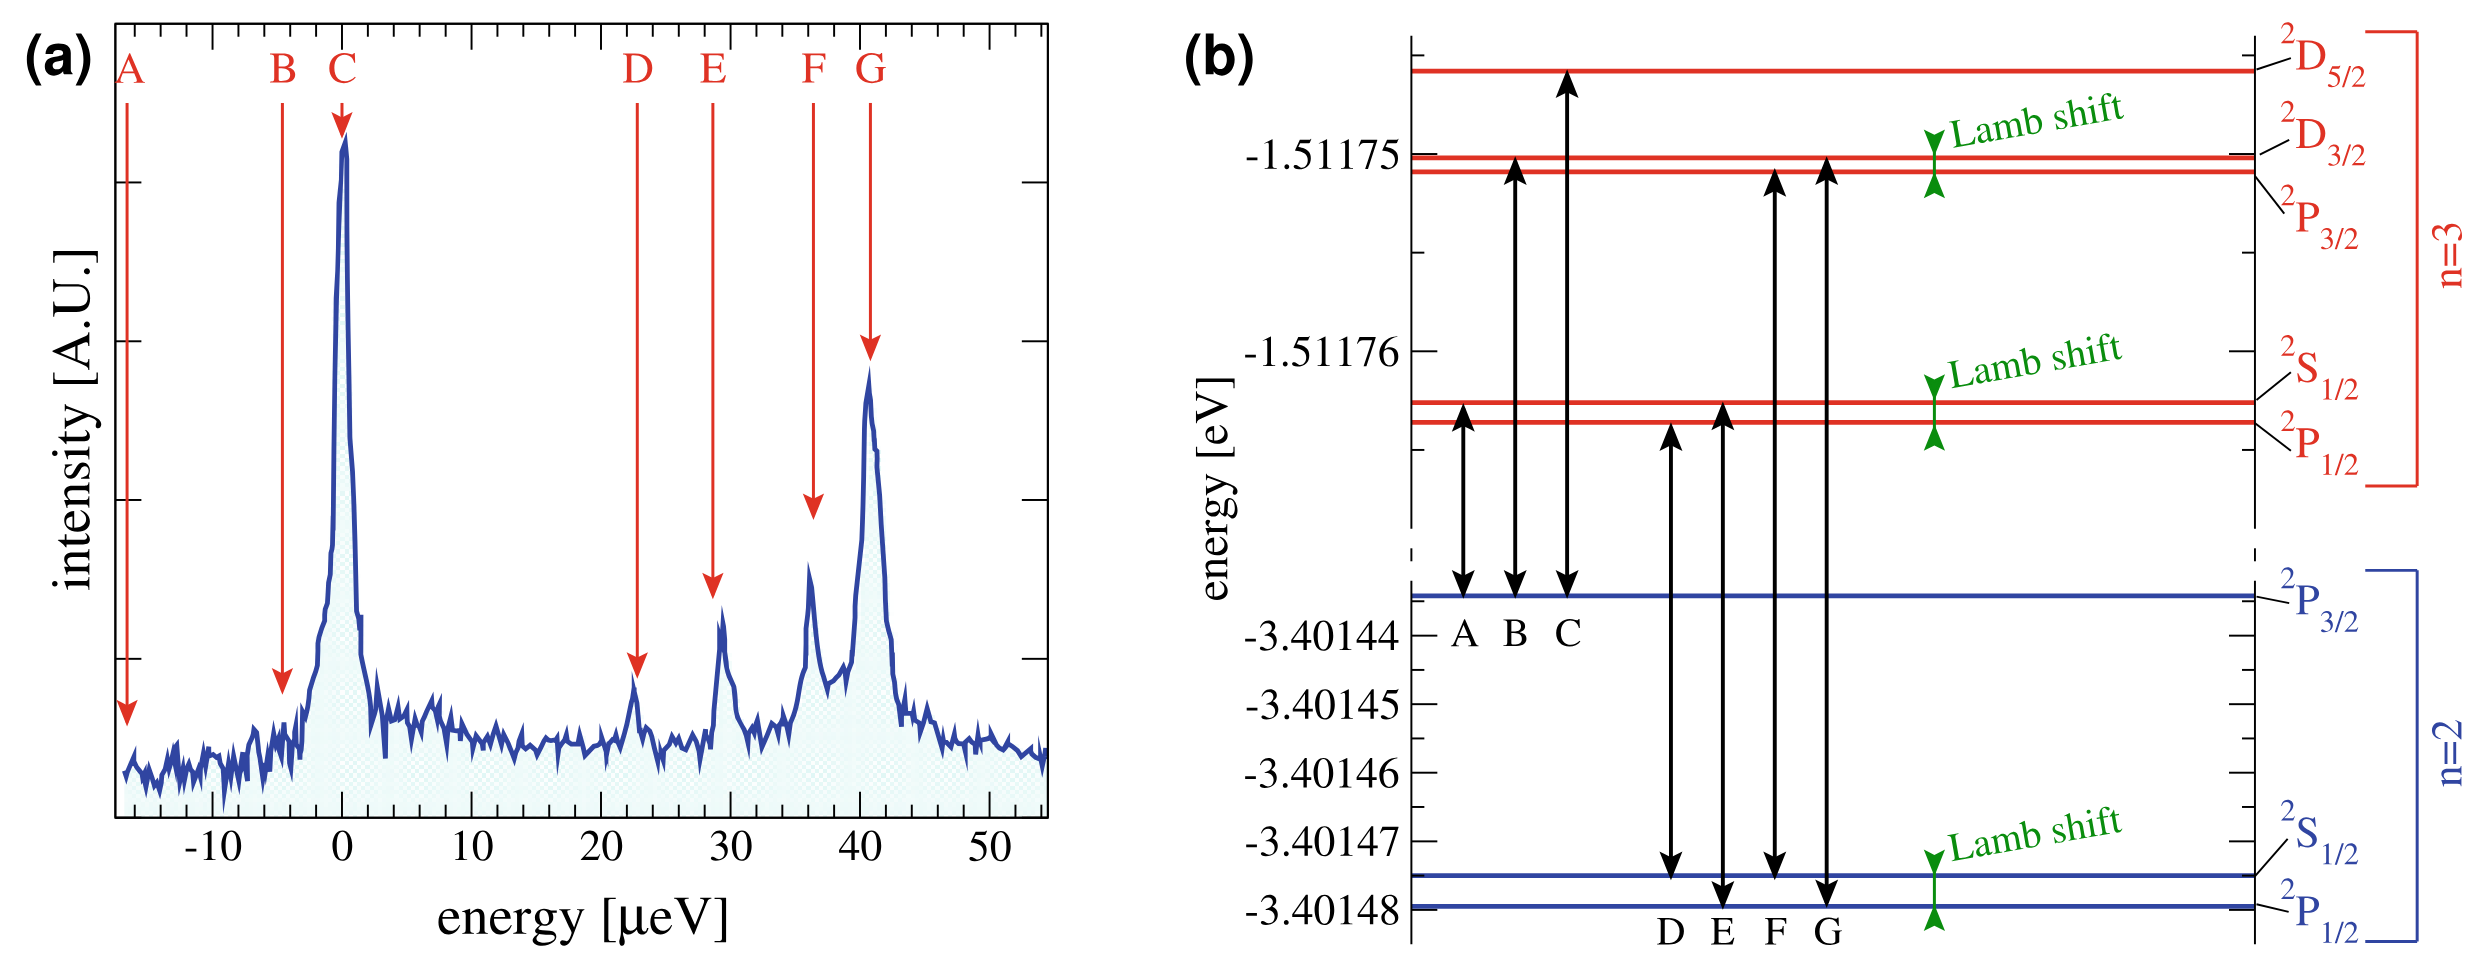
\includegraphics[width = 0.70 \textwidth]{lamb-shift.png}
	\caption{Lamb shift, both theoretical (b) and experimental (a), in the Balmer $ \ch{H}\alpha $ line.}
	\label{img:lamb}
\end{figure}

\section{Struttura iperfine}

Al pari degli elettroni, anche i nuclei hanno un momento angolare di spin $ \ve{I} $, e per molte specie nucleari esso è non-nullo (es.: per il protone $ i = \tfrac{1}{2} $). Per il momento magnetico nucleare sussiste la relazione:
\begin{equation}
	\bs{\mu}_n = g_n \mu_\text{N} \bs{i}
\end{equation}
dove $ \mu_\text{N} \equiv \frac{\hbar q_e}{2m_p} $ è il \textit{magnetone nucleare}. Il valore di $ g_n $ dipende dalla struttura interna del nucleo: ad esempio, per il protone $ g_n \simeq 5.58569 $.\\
Sebbene il campo magnetico nucleare, a parità di distanza, risulti soppresso di $ m_e / m_p \simeq 1 / 1836 $ rispetto a quello elettronico, attraverso questi i momenti magnetici nucleare ed elettronico interagiscono. Dato il fattore $ r^\ell $ in Eq. \ref{eq:1-e-radial}, elettroni con $ \ell > 0 $ hanno probabilità basse di trovarsi vicino al nucleo, dunque l'interazione con essi può essere ignorata; per quanto riguarda gli orbitali $ \ch{S} $, il campo magnetico elettronico è interamente generato dallo spin elettronico $ \ve{S} $ e, analogamente all'interazione spin-orbita, l'interazione tra spin elettronico e spin nucleare è descritta da:
\begin{equation*}
	\mathcal{H}_\text{s-n} = - C \bs{\mu}_n \cdot \bs{\mu}_e = C g_n g_s \mu_\text{N} \mu_\text{B} \bs{i} \cdot \bs{s}
	\qquad \qquad
	C = \frac{2}{3} \frac{1}{4\pi \epsilon_0 c^2} \abs{R_{n,0}(0)}^2 = \frac{2}{3\pi \epsilon_0 c^2} \left( \frac{Z}{an} \right)^3
\end{equation*}
Ricordando che per l'elettrone $ g_s = 2 $, la coupling energy caratteristica risulta essere:
\begin{equation}
	\xi_\text{N} = \frac{4}{3} g_n \frac{Z^3 \alpha^2}{n^3} \frac{m_e}{m_n} E_\text{Ha} \simeq g_n \frac{Z^3}{n^3} \times 1.05\,\mu\text{eV}
\end{equation}
Secondo le regole del momento angolare, $ \ve{I} $ ed $ \ve{S} $ si accoppiano in un \textit{momento angolare atomico} $ \ve{F} = \ve{I} + \ve{S} $, così che per il fattore $ \bs{i} \cdot \bs{s} $ valga, nella coupled basis ($ F^2 $ ed $ F_z $ diagonali), una relazione analoga ad Eq. \ref{eq:sl-coupled-basis}. Ricordando che $ s = \tfrac{1}{2} $, l'interazione tra momenti magnetici nucleare ed elettronico determina uno splitting tra i livelli iperfini $ f = i \pm \tfrac{1}{2} $ pari energeticamente a $ \xi_\text{N} (i \pm \tfrac{1}{2}) $.

\begin{example}{Riga $ 21\,\text{cm} $ dell'idrogeno}{}
	Per $ \ch{^1H} $ si ha $ i = \tfrac{1}{2} $, quindi $ \braket{\bs{i} \cdot \bs{s}} = - \tfrac{3}{4}, \tfrac{1}{4} $ per $ f = 0,1 $ rispettivamente. Nel ground state $ n = 1 $, dunque i due stati iperfini $ f = 0 $ ed $ f = 1 $ risulteranno separati di $ \xi_\text{N} \simeq 5.88\,\mu\text{eV} $: la transizione tra questi livelli sarebbe proibità, poiché $ \Delta \ell = 0 $, ma ha una probabilità non-nulla di avvenire tramite emissione di un fotone con $ \lambda = 2\pi \hbar c \xi_\text{N} \simeq 21\,\text{cm} $ e frequenza $ \nu = \xi_\text{N} (2\pi \hbar)^{-1} \simeq 1.42\,\text{GHz} $. Questa riga spettrale ha valenza storica, in quanto la lunga vita media della transizione (poiché proibita) ne ha permesso la misura della frequenza molto precisa, tant'è che per un periodo è stata usata come standard per l'unità di tempo.
\end{example}

\begin{example}{Struttura iperfine del cesio-137}{}
	Il $ \ch{^{137}Cs} $ è un nuclide con tutte le shell complete ed un elettrone ottico esterno, dunque può essere trattato come un atomo idrogenoide con $ i = \tfrac{7}{2} $ (nuclide dispari-pari). Di conseguenza, per il momento angolare atomico sono possibili solo due valori, dato che $ 3 \le f \le 4 $: la transizioni tra di essi produce un fotone di frequenza $ \nu = 9.192631770 \,\text{GHz} $, e questa riga spettrale e al momento utilizzata come standard per l'unità di tempo.
\end{example}

\section{Transizioni elettroniche}

\subsection{Decadimento spontaneo}

Quando un atomo viene eccitato, esso tenderà a decadere spontaneamente: sperimentalmente, si osserva che non tutte le transizioni procedono allo stesso rate, e ciò può essere spiegato da un'analisi quanto-meccanica dell'interazione del sistema col campo elettromagnetico ambientale. Nell'\textit{approssimazione di dipolo elettrico}\footnotemark, si trova che la probabilità di decadimento radiativo nell'unità di tempo da uno stato iniziale $ \ket{\text{i}} $ ad uno finale $ \ket{\text{f}} $ è:
\begin{equation}
	\gamma_\text{if} = \frac{1}{3\pi \epsilon_0 \hbar^4 c^3} \mathcal{E}_\text{if}^3 \abs{\braket{\text{f} | \ve{d} | \text{i}}}^2
	\label{eq:electron-trans-prob}
\end{equation}
con $ \mathcal{E}_\text{if} \equiv \hbar \omega_\text{if} \defeq E_\text{i} - E_\text{f} $ e $ \ve{d} \equiv - q_e \ve{r} $ l'operatore dipolo elettrico. La dipendenda dall'elemento di matrice $ \braket{\text{f} | \ve{d} | \text{i}} $ impone delle selection rules: le transizioni proibite avvengono con probabilità estremamente inferiori, dato che sono associate a termini di ordine superiore (in $ \alpha $) nell'espansione in multipolo (dipolo magnetico, quadrupolo elettrico, ...).

\footnotetext{Approssimazione valida nel caso in cui la sorgente della radiazione abbia dimensioni molto minori della lunghezza d'onda della radiazione emessa. Essendo $ k = \frac{2\pi}{\lambda} $ e $ \lambda = \frac{hc}{E} $, si ha $ k = \frac{E}{\hbar c} $, dunque tale approssimazione è valida, per $ E \sim 10 - 30 \ev $, se $ k \sim (100 \ang)^{-1} $. Inoltre, si noti che:
\begin{equation}
	\abs{\braket{\text{f} | \ve{p} | \text{i}}}^2 = \abs{\braket{\text{f} | \frac{m}{i\hbar} [\ve{r} , \mathcal{H}] | \text{i}}}^2 = \frac{m^2}{\hbar^2} (E_\text{i} - E_\text{f})^2 \abs{\braket{\text{f} | \ve{r} | \text{i}}}^2 = \frac{m^2}{\hbar^2 q_e^2} \mathcal{E}_\text{if}^2 \abs{\braket{\text{f} | \ve{d} | \text{i}}}^2
	\label{eq:electric-dipole-approx}
\end{equation}}

\begin{theorem}{Electric-dipole selection rule}{}
	Nell'approssimazione di dipolo elettrico per un atomo idrogenoide, le transizioni spontanee ammesse soddisfano:
	\begin{equation}
		\Delta \ell = \pm 1
	\end{equation}

	\tcblower
	
	\begin{proof}
		Esplicitando l'elemento di matrice di $ \ve{d} \equiv -q_e \ve{r} $ in funzione di quello di $ \ve{r} $:
		\begin{equation*}
			\abs{\braket{\text{f} | \ve{r} | \text{i}}}^2 = \abs{\braket{\text{f} | r_x | \text{i}}}^2 + \abs{\braket{\text{f} | r_z | \text{i}}}^2 + \abs{\braket{\text{f} | r_z | \text{i}}}^2
		\end{equation*}
		In funzione delle armoniche sferiche:
		\begin{align*}
			r_x &= r \sin \vartheta \cos \varphi = r \sqrt{\frac{2\pi}{3}} \left[ Y_{1,-1}(\vartheta, \varphi) - Y_{1,1}(\vartheta, \varphi) \right] \\
			r_y &= r \sin \vartheta \sin \varphi = r i \sqrt{\frac{2\pi}{3}} \left[ Y_{1,-1}(\vartheta, \varphi) + Y_{1,1}(\vartheta, \varphi) \right] \\
			r_z &= r \sqrt{\frac{4\pi}{3}} Y_{1,0}(\vartheta, \varphi)
		\end{align*}
		Ne segue che:
		\begin{equation*}
			\abs{\braket{\text{f} | \ve{r} | \text{i}}}^2 = \abs{\braket{\text{f} | r | \text{i}}}^2 \frac{4\pi}{3} \left[ \abs{\braket{\text{f} | Y_{1,-1} | \text{i}}}^2 + \abs{\braket{\text{f} | Y_{1,0} | \text{i}}}^2 + \abs{\braket{\text{f} | Y_{1,1} | \text{i}}}^2 \right]
		\end{equation*}
		Esplicitando in termini della funzione d'onda elettronica:
		\begin{equation*}
			\begin{split}
				\abs{\braket{n_\text{f} , \ell_\text{f} , m_\text{f} | \ve{d} | n_\text{i} , \ell_\text{i} , m_\text{i}}}^2
				& = q_e^2 \abs{\int_0^\infty \dd r\, r^2 R_{n_\text{f} , \ell_\text{f}}(r) R_{n_\text{i} , \ell_\text{i}}(r)}^2 \times \\
				& \times \frac{4\pi}{3} \sum_{m = -1,0,1} \abs{\int_0^\pi \dd \vartheta \, \sin \vartheta \int_0^{2\pi} \dd \varphi \, Y_{\ell_\text{f} , m_\text{f}}^*(\vartheta,\varphi) Y_{1,m}(\vartheta,\varphi) Y_{\ell_\text{i} , m_\text{i}}(\vartheta,\varphi)}^2
			\end{split}
		\end{equation*}
		L'integrale spaziale contribuisce soltanto allo smorzamento delle transizioni con $ \abs{n_\text{i} - n_\text{f}} $ grande, mentre la selection rule è imposta dall'integrale angolare: si noti che esso rappresenza l'overlap angolare tra $ Y_{\ell_\text{f} , m_\text{f}} $ e $ Y_{1,m} Y_{\ell_\text{i} , m_\text{i}} $, ma quest'ultimo può essere scomposto (secondo la decomposizione di Clebsch-Gordan) nella somma di stati con $ \ell = \abs{\ell_\text{i} - 1}, \ell_\text{i}, \ell_\text{i} + 1 $, dunque l'elemento di matrice è non-nullo sono per $ \ell_\text{f} = \ell $. Inoltre, si noti che l'integrale si annulla per $ \ell_\text{f} = \ell_\text{i} $: in tal caso, la parità dell'integranda sarebbe $ (-1)^{\ell_\text{i}} (-1)^1 (-1)^{\ell_\text{i}} = -1 $, dunque il suo integrale su tutto l'angolo solido è nullo. Gli unici valori possibili sono dunque $ \ell_\text{f} = \ell_\text{i} \pm 1 $, ovvero la selection rule cercata.
	\end{proof}
\end{theorem}

Essendo l'operatore dipolo elettrico associato a $ \ell = 1 $, si ha che $ m = -1,0,1 $; di conseguenza, si ottiene una selection rule anche sulla proiezione del momento angolare orbitale:
\begin{equation}
	\Delta m = 0, \pm 1
\end{equation}
Inoltre, dato che $ \ve{d} $ agisce come l'identità sullo spazio degli spin, si hanno:
\begin{equation}
	\Delta s = 0
	\qquad \qquad
	\Delta m_s = 0
	\label{eq:1-e-el-dip-tr-spin}
\end{equation}
È anche possibile esprimere la selection rule sulla base accoppiata, ottenendo:
\begin{equation}
	\Delta j = 0 , \pm 1
	\qquad \qquad
	\Delta m_j = 0 , \pm 1
\end{equation}
Una volta determinate le transizioni possibili, si può dare una stima del decay rate dall'Eq. \ref{eq:electron-trans-prob}, usando $ \mathcal{E}_\text{if} \simeq Z^2 E_\text{Ha} $ e $ \abs{\braket{\text{f} | \ve{d} | \text{i}}} = q_e a_0 / Z $:
\begin{equation*}
	\gamma_\text{if} = \frac{\mathcal{E}_\text{if}^3 \abs{\braket{\text{f} | \ve{d} | \text{i}}}^2}{3\pi \epsilon_0 \hbar^4 c^3} \simeq \frac{Z^4 E_\text{Ha}^2}{\epsilon_0 \hbar^4 c^3} \hbar \omega_\text{if} \frac{q_e^2 a_0^2}{Z^2} \simeq \frac{e^2 Z^2}{(\hbar c)^3} e^4 \omega_\text{if} = Z^2 \alpha^3 \omega_\text{if}
\end{equation*}
dato che $ E_\text{Ha} a_0 = e^2 $ e $ \alpha = e^2 / (\hbar c) $. Per un atomo idrogenoide $ \omega_\text{if} \simeq Z^2 \cdot 10^{16} \,\text{Hz} $, dunque si trova un tempo di decadimento dell'ordine $ \gamma_\text{if}^{-1} \simeq Z^{-4} \,\text{ns} $.

\begin{example}{Doppietto giallo del sodio}{}
	L'atomo di sodio presenta 11 elettroni: 10 interni in shell complete ed 1 esterno in 3s. Come in tutti gli altri atomi alcalini, l'elettrone esterno si trova più lontano dal nucleo rispetto alle shell interne ed è chiamato \textit{elettrone ottico}, poiché tipicamente le sue transizioni cadono nel visibile. Il potenziale a cui è soggetto l'elettrone ottico può essere visto come Coulombiano con un $ Z_\text{eff} $ efficacie: a grandi distanze dal nucleo $ Z_\text{eff} \simeq Z - (Z-1) = 1 $, mentre avvicinandosi ad esso $ Z_\text{eff} = Z_\text{eff}(r) $, il che rompe la degenerazione accidentale (l'energia è $ E = E(n,\ell) $). \\
	Nel caso del sodio, il tipico doppietto giallo del suo spettro d'emissione è dovuto alla transizione ottica ($ \Delta \ell = \pm 1 $) più piccola possibile per l'elettrone ottico, ovvero $ \text{3p} \rightarrow \text{3s} $ ($ \Delta E \sim 2\ev $). In particolare, sono presenti due righe a causa dell'interazione spin-orbita ($ \Delta E \sim 2.1 \,\text{meV} $), poiché le transizioni possibili sono due: $ \ch{^3P}_{3/2} \rightarrow \ch{^3S}_{1/2} $ ($ \lambda = 589.0 \,\text{nm} $) e $ \ch{^3P}_{1/2} \rightarrow \ch{^3S}_{1/2} $ ($ \lambda = 589.6 \,\text{nm} $).
\end{example}

\subsection{Decadimento stimolato}

In generale, un sistema immerso in un campo elettromagnetico descritto dai potenziali $ \phi $ ed $ \ve{A} $ è descritto dall'Hamiltoniana:
\begin{equation}
	\mathcal{H} = \frac{1}{2m} \left( \ve{p} - \frac{q}{c} \ve{A} \right)^2 + q \phi
\end{equation}
Nel caso dell'atomo idrogenoide:
\begin{equation}
	\mathcal{H} = \frac{1}{2m_e} \left( \ve{p} + \frac{e}{c} \ve{A} \right)^2 + \frac{1}{2M} \left( \ve{P} - \frac{Ze}{c} \ve{A} \right)^2 - \frac{Ze}{\abs{\ve{r} - \ve{R}}}
\end{equation}
Trascurando $ \frac{1}{M} \ll \frac{1}{m_e} $, ponendo $ \ve{R} = \ve{0} $ e scegliendo un gauge $ [\nabla , \ve{A}] = 0 $:
\begin{equation*}
	\begin{split}
		\mathcal{H}
		& \simeq \frac{1}{2m_e} \left( \ve{p} + \frac{e}{c} \ve{A} \right)^2 - \frac{Ze}{r} = \frac{1}{2m_e} \left[ -\hbar^2 \lap - i \frac{\hbar e}{c} (\nabla \cdot \ve{A} + \ve{A} \cdot \nabla) + \frac{e^2}{c^2} \ve{A}^2 \right] - \frac{Ze}{r} \\
		& = \frac{\hbar^2}{2m_e} \left[ -\lap - 2i \frac{\alpha}{e} \ve{A} \cdot \nabla + \frac{\alpha^2}{e^2} \ve{A}^2 \right] - \frac{Ze}{r} = \underbrace{- \frac{\hbar^2}{2m_e} \lap - \frac{Ze}{r}}_{\mathcal{H}_0} \underbrace{- i \frac{\hbar^2}{m_e} \frac{\alpha}{e} \ve{A} \cdot \nabla}_{V} + \underbrace{\frac{\hbar^2}{2m_e} \frac{\alpha^2}{e^2} \ve{A}^2}_{\sim \, \alpha^2}
	\end{split}
\end{equation*}
L'ultimo termine può essere trascurato, dunque il problema può essere trattato perturbativamente al prim'ordine (nell'approssimazione di campo debole). Per semplificare la trattazione, si adottano le unità atomiche $ \hbar = m_e = e = 1 , c = \alpha^{-1} \simeq 137 $:
\begin{equation}
	\mathcal{H} \simeq - \frac{1}{2} \lap - \frac{Z}{r} - i \alpha \ve{A} \cdot \nabla
\end{equation}
La dipendenza temporale degli autostati di $ \mathcal{H} $ non è più banale, in quanto la perturbazione determina una dipendenza temporale:
\begin{equation}
	\psi(t,r) = \sum_{n \in \N} c_n(t) e^{-i E_n t} \psi_n(r)
	\label{eq:1-e-pert-autof}
\end{equation}
dove $ \psi_n(r) $ sono gli stati stazionari di $ \mathcal{H}_0 $ e al prim'ordine:
\begin{equation}
	c_n(t) \simeq c_n^{(0)} + c_n^{(1)}(t)
	\label{eq:1-e-pert-coeff}
\end{equation}

\begin{proposition}{Coefficienti perturbativi}{}
	Per un potenziale del tipo:
	\begin{equation}
		\ve{A}(t,\ve{r}) = \ve{A}_0 e^{i (\ve{k}_0 \cdot \ve{r} - \omega_0 t + \varphi_0)} + \text{c.c.} = 2 \ve{A}_0 \cos (\ve{k}_0 \cdot \ve{r} - \omega_0 t + \varphi_0)
	\end{equation}
	i coefficienti nello sviluppo perturbativo per una transizione tra due stati stazionari $ \ket{n} , \ket{m} $ sono:
	\begin{equation}
		\begin{split}
			c_n^{(1)}(t) = - \alpha t \ve{A}_0 \cdot \bigg[
			& \ve{M}_{nm}(\ve{k}_0) \exp \left( i \frac{\omega_{nm} - \omega_0}{2} t + i \varphi_0 \right) \sinc \left( \frac{\omega_{nm} - \omega_0}{2} t \right) + \\
			& \qquad - \ve{M}_{mn}^*(\ve{k}_0) \exp \left( i \frac{\omega_{nm} + \omega_0}{2} t + i \varphi_0 \right) \sinc \left( \frac{\omega_{nm} + \omega_0}{2} t \right) \bigg]
			\label{eq:1-e-big-coeff}
		\end{split}
	\end{equation}
	con $ \ve{M}_{nm}(\ve{k}_0) \equiv \braket{n | e^{i \ve{k}_0 \cdot \ve{r}} \nabla | m} $.

	\tcblower

	\begin{proof}
		L'equazione di Schrödinger per l'autofunzione \ref{eq:1-e-pert-autof} diventa:
		\begin{equation*}
			\sum_{m \in \N} c_m(t) e^{-i E_m t} \mathcal{H} \psi_m(r) = i \sum_{m \in \N} \left[ \frac{dc_m(t)}{dt} - i E_m c_m(t) \right] e^{-i E_m t} \psi_m(r)
		\end{equation*}
		Moltiplicando a sinistra per $ \psi_n^*(r) $ ed integrando su tutto lo spazio:
		\begin{equation*}
			\sum_{m \in \N} c_m(t) e^{-i E_m t} \left( \delta_{nm} + \braket{n | V | m} \right) = \sum_{m \in \N} \left[ i \frac{dc_m(t)}{dt} + E_m c_m(t) \right] e^{-i E_m t} \delta_{nm}
		\end{equation*}
		Semplificando, si trova:
		\begin{equation*}
			\frac{dc_n(t)}{dt} = -i \sum_{m \in \N} c_m(t) e^{i \mathcal{E}_{nm} t} \braket{n | V | m}
		\end{equation*}
		Dall'Eq. \ref{eq:1-e-pert-coeff}, dato che $ c_n^{(1)} \ll c_n^{(0)} $:
		\begin{equation*}
			\frac{dc_n^{(1)}(t)}{dt} = -i \sum_{k \in \N} c_k^{(0)}(t) e^{i \mathcal{E}_{nk} t} \braket{n | V | k}
		\end{equation*}
		Per uno stato iniziale stazionario $ \ket{m} $ si ha $ c_k^{(0)} = \delta_{km} $, dunque:
		\begin{equation*}
			\frac{dc_n^{(1)}(t)}{dt} = -i e^{i \mathcal{E}_{nm} t} \braket{n | V | m} = - e^{i \mathcal{E}_{nm} t} \alpha \ve{A}_0 \cdot \left[ \braket{n | e^{i\ve{k}_0 \cdot \ve{r}} \nabla | m} e^{-i \omega_0 t + \varphi_0} + \text{c.c.} \right]
		\end{equation*}
		Essendo $ \nabla $ anti-hermitiano, $ \ve{M}_{nm}^*(\ve{k}_0) = - \ve{M}_{mn}(\ve{k}_0) $, ovvero:
		\begin{equation*}
			\frac{dc_n^{(1)}(t)}{dt} = - \alpha \ve{A}_0 \cdot \left[ \ve{M}_{nm}(\ve{k}_0) e^{i (\omega_{nm} - \omega_0) t + i \varphi_0} - \ve{M}_{mn}^*(\ve{k}_0) e^{i (\omega_{nm} + \omega_0) t - i \varphi_0} \right]
		\end{equation*}
		Integrando:
		\begin{equation*}
			\int_0^t dt' e^{i \beta t'} = \frac{e^{i\beta t} - 1}{i \beta} = \frac{i (1 - \cos \beta t) + \sin \beta t}{\beta} = \frac{2}{\beta} e^{i \beta \frac{t}{2}} \sin \left( \beta \tfrac{t}{2} \right) = \frac{t e^{i\beta \frac{t}{2}} \sin \left( \beta \frac{t}{2} \right)}{\beta \frac{t}{2}}
		\end{equation*}
		Utilizzando questo risultato per risolvere l'ODE per $ c_n^{(1)}(t) $ si ottiene la tesi.
	\end{proof}
\end{proposition}

Si ottiene quindi che, per un sistema inizialmente in uno stato stazionario $ \ket{m} $:
\begin{equation}
	\psi(t,r) = \psi_m(r) + \sum_{n \in \N} c_{nm}(t) e^{- i E_n t} \psi_n(r)
\end{equation}
con $ c_{nm}(t) \equiv c_n^{(1)}(t) $ come in Eq. \ref{eq:1-e-big-coeff}. La probabilità di transizione da $ \ket{m} $ a $ \ket{n} $, con $ n \neq m $, sarà dunque $ P_{nm}(t) = \abs{c_{nm}(t)}^2 $.

\paragraph{Risonanza}

Essendo $ \omega_0 $ la pulsazione della radiazione incidente, in base al valore di $ \omega_{nm} $ (differenza tra i due livelli energetici) si hanno due possibili risonanze (a seconda di quale termine domina in Eq. \ref{eq:1-e-big-coeff}):
\begin{itemize}
	\item $ \omega_{nm} \approx \omega_0 $: domina il primo termine, ovvero si ha risonanza per il processo di assorbimento (eccitamento) con transizione da $ \omega_m $ a $ \omega_n = \omega_m + \omega_0 $;
	\item $ \omega_{nm} \approx - \omega_0 $: domina il secondo termine, ovvero si ha risonanza per il processo di emissione (decadimento) con transizione da $ \omega_m $ a $ \omega_n = \omega_m - \omega_0 $.
\end{itemize}
Inoltre, si noti che $ \sinc{x} \rightarrow 0 $ per $ x \rightarrow \infty $, dunque col passare del tempo le probabilità di transizione per $ n \neq m $ tendono ad annullarsi; ciò è legato alla natura della radiazione emessa: inizialmente essa è non-monocromatica, ma col passare del tempo tende a diventare sempre più monocromatica.

\paragraph{Golden rule di Fermi}

È possibile definire la probabilità di transizione per unità di tempo sia nel caso dell'assorbimento che in quello dell'emissione:
\begin{align*}
	P_\text{a}(t) &= \abs{c_{nm}(t)}^2 \simeq \alpha^2 t^2 A_0^2 \abs{\bs{\epsilon} \cdot \ve{M}_{nm}(\ve{k}_0)}^2 \sinc^2 \left( \tfrac{\omega_{nm} - \omega_0}{2} t \right) \sim 2\pi \alpha^2 t A_0^2 \abs{\bs{\epsilon} \cdot \ve{M}_{nm}(\ve{k}_0)}^2 \delta(\tfrac{\omega_{nm} - \omega_0}{2}) \\
	P_\text{e}(t) &= \abs{c_{nm}(t)}^2 \simeq \alpha^2 t^2 A_0^2 \abs{\bs{\epsilon} \cdot \ve{M}_{mn}^*(\ve{k}_0)}^2 \sinc^2 \left( \tfrac{\omega_{nm} + \omega_0}{2} t \right) \sim 2\pi \alpha^2 t A_0^2 \abs{\bs{\epsilon} \cdot \ve{M}_{mn}^*(\ve{k}_0)}^2 \delta(\tfrac{\omega_{nm} + \omega_0}{2})
\end{align*}
dove $ \bs{\epsilon} = \ve{A}_0 / A_0 $ è la polarizzazione della radiazione incidente e $ \delta(x) = \frac{1}{2\pi} \lim_{t \rightarrow \infty} t \sinc^2(xt) $. Definendo l'intensità della radiazione incidente come $ I_0 \equiv A_0^2 \omega_0^2 / (2\pi c) $, si ottiene la golden rule di Fermi:
\begin{align*}
	P_\text{a}(t) &\simeq 4\pi \alpha^2 t \abs{\bs{\epsilon} \cdot \ve{M}_{nm}(\ve{k}_0)}^2 \frac{I_0}{\omega_0^2} \delta(\omega_{nm} - \omega_0) \\
	P_\text{e}(t) &\simeq 4\pi \alpha^2 t \abs{\bs{\epsilon} \cdot \ve{M}_{mn}^*(\ve{k}_0)}^2 \frac{I_0}{\omega_0^2} \delta(\omega_{nm} + \omega_0)
\end{align*}
Si noti che l'unico termine distinto è la $ \delta $ di conservazione dell'energia, la quale può essere scritta in maniera unificata come $ \delta(\omega_\text{f} - \omega_\text{i}) $. Inoltre, si vede che la probabilità di transizione diverge alla risonanza: questo però non è un problema, in quanto non esistono sorgenti puramente monocromatiche, in quanto dovrebbero emettere per un tempo infinito; più realisitcamente, si ha una distribuzione d'intensità attorno a $ \omega_0 $, così da scrivere:
\begin{equation*}
	\frac{I_0}{\omega_0^2} \delta(\omega_{nm} \pm \omega_0) \longrightarrow \int_{-\infty}^{+\infty} d\omega\, \frac{I(\omega)}{\omega^2} \delta(\omega_{nm} \pm \omega_0) = \frac{I(\omega_{nm})}{\omega_{nm}^2}
\end{equation*}
Utilizzando l'approssimazione di dipolo elettrico Eq. \ref{eq:electric-dipole-approx}, si trova che il rate di transizione $ \gamma_\text{if} \equiv P_\text{if} / t $ può essere scritto come:
\begin{equation*}
	\gamma_\text{if} = 4\pi \alpha^2 \abs{\braket{\text{f} | e^{i \ve{k}_0 \cdot \ve{r}} \nabla | \text{i}}}^2 \frac{I(\omega_\text{if})}{\omega_\text{if}^2} \simeq 4\pi \alpha^2 \abs{\braket{\text{f} | \ve{p} | \text{i}}}^2 \frac{I(\omega_\text{if})}{\omega_\text{if}^2} = 4\pi \alpha^2 \omega_\text{if}^2 \abs{\braket{\text{f} | \ve{d} | \text{i}}}^2 \frac{I(\omega_\text{if})}{\omega_\text{if}^2}
\end{equation*}
Si trova dunque:
\begin{equation}
	\gamma_\text{if} = 4\pi \alpha^2 I(\omega_\text{if}) \abs{\braket{\text{f} | \ve{d} | \text{i}}}^2
\end{equation}
A differenza dell'emissione spontanea, che è $ \sim \mathcal{E}_\text{if}^3 $, quella stimolata è $ \sim \mathcal{E}_\text{if}^2 $, dunque l'emissione spontanea diventa più probabile di quella stimolata all'aumentare della differenza energetica.

\section{Campo magnetico esterno}

Maggiori informazioni su una specie atomica possono essere ricavate immergendo il campione in un campo magnetico uniforme e studiandone lo spettro. Il momento magnetico atomico totale può essere scritto come:
\begin{equation}
	\bs{\mu} = \bs{\mu}_\ell + \bs{\mu}_s = - \mu_\text{B} ( g_\ell \bs{\ell} + g_s \bs{s}) \simeq - \mu_\text{B} (\bs{\ell} + 2 \bs{s})
\end{equation}
L'Hamiltoniana di coupling con un campo magnetico esterno, WLOG $ \ve{B} = B \hat{\ve{e}}_z $, è:
\begin{equation}
	\mathcal{H}_\text{magn} = - \bs{\mu} \cdot \ve{B} = \mu_\text{B} B (\ell_z + 2s_z)
\end{equation}
Si vede che $ \mathcal{H}_\text{magn} $ è diagonalizzabile nella uncoupled basis $ \ket{\ell, m, s, m_s} $, mentre $ \mathcal{H}_\text{s-o} $ lo è nella coupled basis $ \ket{\ell, s, j, m_j} $: dato che $ [\mathcal{H}_\text{magn} , \mathcal{H}_\text{s-o}] \neq 0 $, essi non sono simultaneamente diagonalizzabili, ma vanno diagonalizzati di volta in volta in ogni sottospazio $ (2\ell + 1)(2s + 1) $-dimensionale a $ n,\ell,s $ fissati.
È però possibile studiare i casi limite per le energie caratteristiche $ \mu_\text{B} B $ e $ \xi $.

\subsection{Limite Paschen-Back}

Nel limite $ \mu_\text{B} B \gg \xi $ in cui domina il campo magnetico esterno, la diagonalizzazione è diretta poiché si usa la uncoupled basis:
\begin{equation}
	\Delta E_\text{magn}(m,m_s) = \braket{m,m_s | \mathcal{H}_\text{magn} | m,m_s} = \mu_\text{B} B (m + 2m_s)
\end{equation}
mentre la correzione dovuta a $ \mathcal{H}_\text{s-o} $ può essere trattata perturbativamente. \\
Il valore di $ B $ per cui si può effettuare questa approssimazione dipende dall'atomo considerato e dal livello energetico: ad esempio, considerando la shell $ \text{2p} $, per $ \ch{H} $ si ha $ B \gg 0.5 \,\text{T} $, mentre per $ \ch{He}^+ $ si ha $ B \gg 8 \,\text{T} $, a causa della dipendenza da $ Z^4 $ in Eq. \ref{eq:1-e-int-spin-orb}.

\subsection{Limite Zeeman}

Il limite $ \mu_\text{B} B \ll \xi $ in cui domina l'interazione spin-orbita è quello più comune e in esso la simmetria sferica subisce solo una debole perturbazione. Gli stati $ \ket{\ell,s,j,m_j} $ nella coupled basis sono dunque autostati approssimati di $ \mathcal{H}_\text{s-o} + \mathcal{H}_\text{magn} $, mentre la correzione al prim'ordine dell'energia è:
\begin{equation}
	\Delta E_\text{magn}(j,m_j) \simeq \braket{j,m_j | \mathcal{H}_\text{magn} | j,m_j} = g_j \mu_\text{B} B m_j
\end{equation}
dove $ g_j $ è il fattore di Landé (Eq. \ref{eq:lande-g-factor}).

\subsection{Linee spettrali}

Sperimentalmente, si confermano le considerazioni teoriche sia esatte che approssimate. Prendendo ad esempio un campione di $ \ch{H} $, applicando un campo magnetico sufficientemente potente si osserva una triplicazione delle linee spettrali ($ \Delta m = 0, \pm 1 $), in accordo con l'effetto Paschen-Back, mentre applicando un campo magnetico debole si osserva l'effetto Zeeman (Fig. \ref{zeeman-effect}).

\begin{figure}
	\centering
	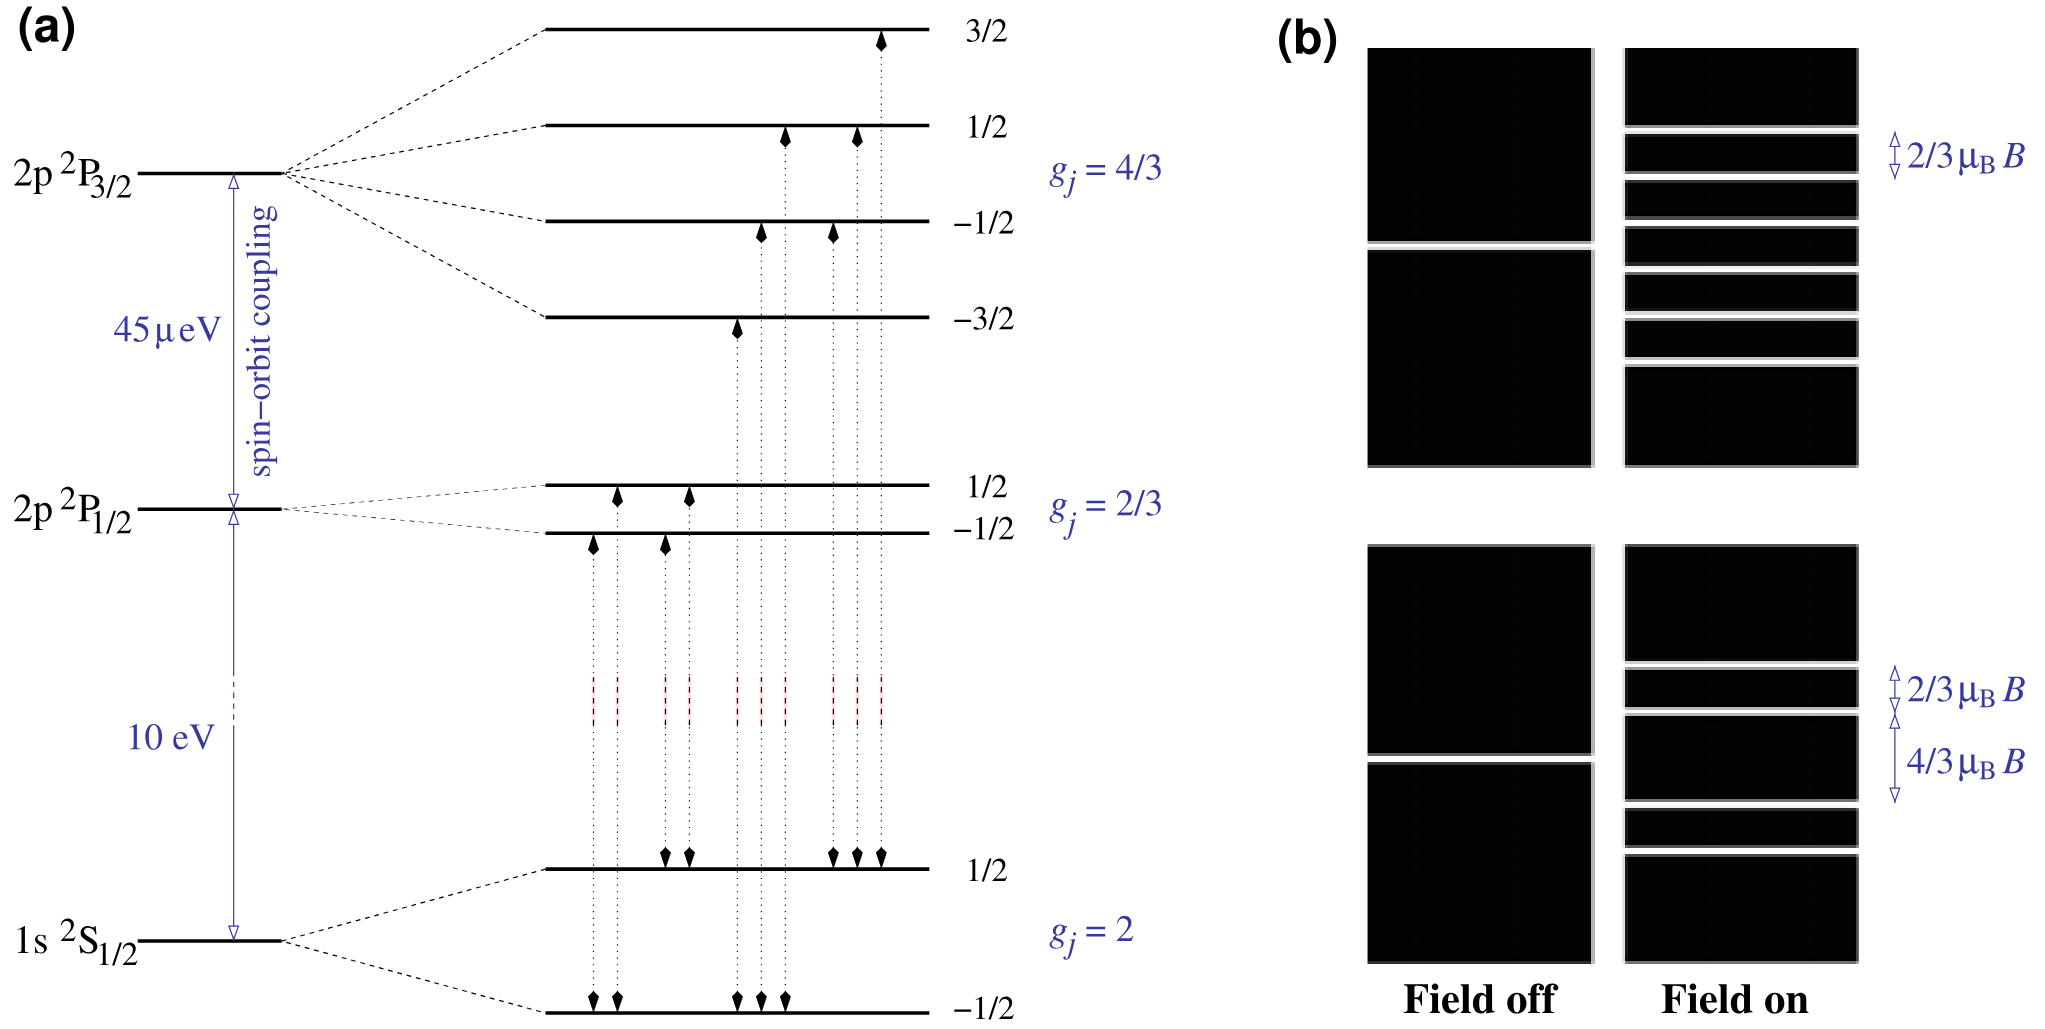
\includegraphics[width = 0.85 \textwidth]{zeeman-effect.png}
	\caption{Zeeman split of the lowest Lyman line of $ \ch{H} $.}
	\label{zeeman-effect}
\end{figure}

Nel regime intermedio $ \mu_\text{B} B \sim \xi $, nessuna delle due basi riesce a dare una descrizione accurata dei livelli energetici. Ad esempio, Fig. \ref{mag-field-int} mostra lo splitting pattern dei 6 stati $ \ch{^2P} $ in funzione dell'intensità del campo magnetico.

\begin{figure}[!b]
	\centering
	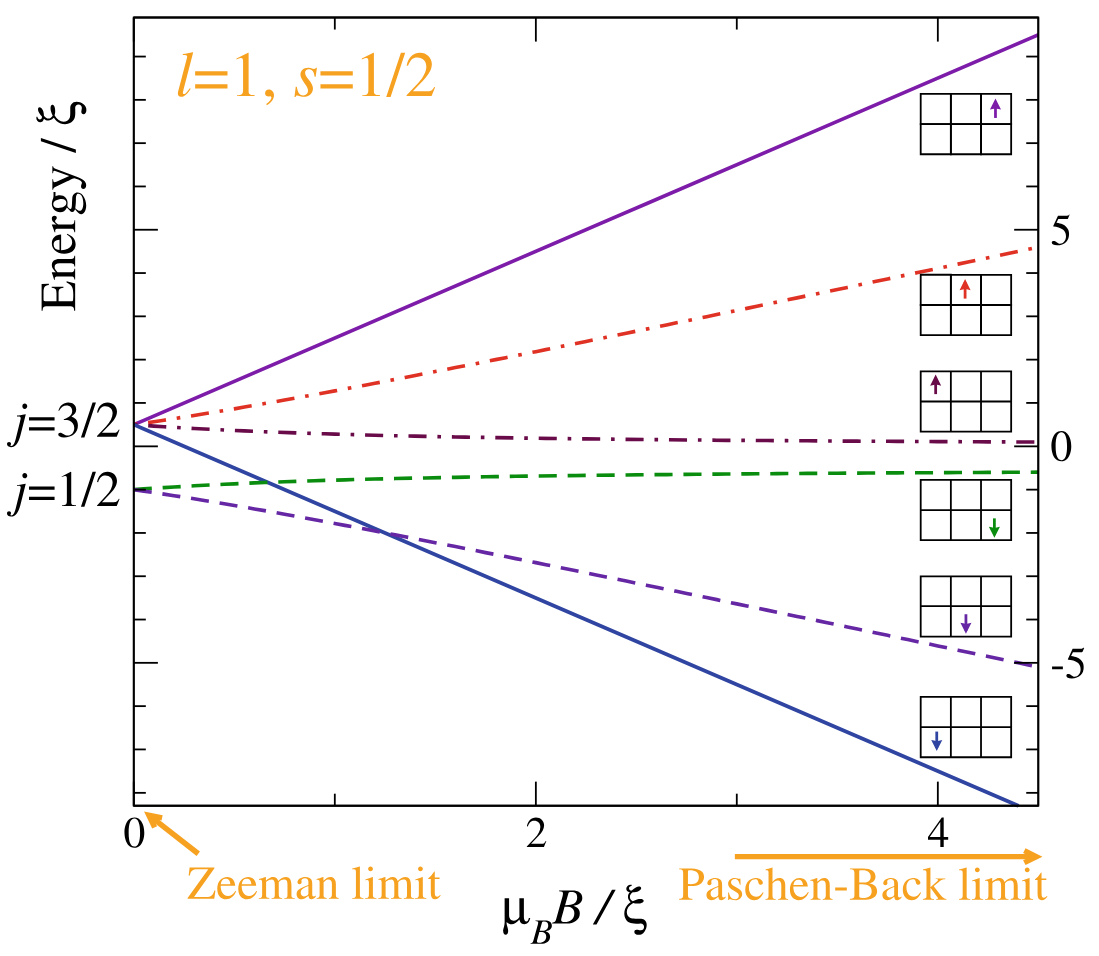
\includegraphics[width = 0.50 \textwidth]{mag-field-int.png}
	\caption{Combined spin-orbit and magnetic splittings of $ \ch{^2P} $.}
	\label{mag-field-int}
\end{figure}












\chapter{Atomi a Più Elettroni}
\selectlanguage{italian}

La trattazione degli atomi a molti elettroni (Many-Electron Atoms) è resa non banale dall'interazione elettrone-elettrone, la quale rende impossibile la risoluzione esatta del problema\footnotemark. È dunque necessario adottare alcune semplificazioni.

\footnotetext{La funzione d'onda di ciascun elettrone dipende da tre variabili spaziali, dunque, discretizzando ciascuna di esse in una griglia di 10 numeri reali, la descrizione di un sistema a $ N $ elettroni richiede di trattare $ (10^3)^N $ numeri reali: già per $ N = 4 $ ciò necessiterebbe di qualche Tb, mentre per $ N = 27 $ si raggiunge l'ordine di grandezza del numero totale di atomi nell'Universo. La trattazione numerica del problema è dunque impossibile.}

\section{Approssimazione a particelle indipendenti}

È possibile trovare soluzioni approssimate per MEAs costruendo il relativo spazio di Hilbert a partire dagli stati single-particle.

\subsection{Particelle identiche}

Gli elettroni sono particelle indistinguibili tra loro, dunque è necessario ricordare le proprietà dei sistemi quantistici di particelle identiche. \\
Dato un sistema di $ N $ particelle identiche, ciascuna descritta da uno spazio di Hilbert $ \hilb $, il sistema totale sarà descritto da un sottospazio del prodotto diretto di tali spazi. In particolare, definendo l'operatore di scampio $ \pi_{ij} $ che scambia le particelle $ i \leftrightarrow j $, dato che $ \pi_{ij}^2 $ si ha che i suoi autovalori possibili sono $ \pm 1 $: stati $ \pi_{ij} \ket{\psi} = + \ket{\psi} $ sono detti \textit{stati bosonici}, sono simmetrici per scambio di particelle e descrivono sistemi di spin intero; stati $ \pi_{ij} \ket{\psi} = - \ket{\psi} $ sono detti \textit{stati fermionici}, sono antisimmetrici per scambio di particelle e descrivono sistemi di spin semi-intero. La definizione degli stati bosonici/fermionici a partire dagli stati single-particle è dunque data rispettivamente da:
\begin{equation}
	\ket{\alpha_1 , \dots , \alpha_N}^\text{(s)} \defeq \frac{1}{\sqrt{N!}} \sum_{\pi \in S^N} \ket{\alpha_{\pi(1)} , \dots , \alpha_{\pi(N)}}
\end{equation}
\begin{equation}
	\ket{\alpha_1 , \dots , \alpha_N}^\text{(a)} \defeq \frac{1}{\sqrt{N!}} \sum_{\pi \in S^N} (-1)^{\{\pi\}} \ket{\alpha_{\pi(1)} , \dots , \alpha_{\pi(N)}}
\end{equation}
dove $ \{\pi\} $ è il carattere della permutazione e $ \alpha_n $ indica il set completo di quantum numbers dell'$ n $-esima particella. Come si può vedere, il principio d'esclusione di Pauli discende banalmente da queste definizioni: un sistema bosonico non ha restrizioni sui quantum numbers dei singoli bosoni che lo compongono, mentre un sistema fermionico, dato il fattore $ (-1)^{\{\pi\}} $, risulta avere $ \ket{\psi} = 0 $ se si considerano due fermioni con gli stessi quantum numbers.

\begin{example}{Identicità degli atomi}{}
	Si consideri un atomo di $ \ch{^3He} $: esso è composto da 2 protoni, 1 neutrone e 2 elettroni, dunque overall è un sistema fermionico: se si scambiano tra loro due tali atomi, si ottiene un fattore $ (-1)\cdot(-1) = +1 $ per i protoni, idem per gli elettroni, e $ (-1) $ per i neutroni, risultando in un fattore totale $ (-1) $. \\
	D'altro canto, un atomo di $ \ch{^{238}U} $, composto da 92 protoni, 146 neutroni e 92 elettroni, è un sistema bosonico per un ragionamento analogo. \\
	In generale, atomi con $ A + Z $ pari sono bosoni, mentre atomi con $ A + Z $ dispari sono fermioni.
\end{example}

L'antisimmetria per scambio dei sistemi a molti elettroni ne condiziona fortemente al dinamica, in quanto la repulsione tra elettroni data dall'antisimettrizzazione della funzione d'onda è spesso più efficace della repulsione elettromagnetica tra di essi: senza antisimmetria, gli elettroni nel ground state occuperebbero tutti la shell $ \text{1s} $.

\subsubsection{Funzione d'onda fermionica}

Si consideri un sistema di $ N $ fermioni, ciascuno descritto da uno spazio di Hilbert con ket base $ \ket{w_n} = \ket{\ve{r}_n , \sigma_n} $ di posizione e spin.

\begin{theorem}{Determinante di Slater}{}
	La base dello spazio di Hilbert di un sistema di $ N $ fermioni è data dal \textit{determinante di Slater}:
	\begin{equation}
		\Psi_{\alpha_1 , \dots , \alpha_N}(w_1 , \dots , w_N) = \frac{1}{\sqrt{N!}}
		\begin{vmatrix}
			\psi_{\alpha_1}(w_1) & \dots & \psi_{\alpha_1}(w_N) \\
			\vdots & \ddots & \vdots \\
			\psi_{\alpha_N}(w_1) & \dots & \psi_{\alpha_N}(w_N)
		\end{vmatrix}
	\end{equation}

	\tcblower

	\begin{proof}
		Essendo lo spazio di Hilbert totale $ \hilb^\text{(a)} $, la funzione d'onda dello stato fermionico generico $ \ket{\alpha_1 , \dots , \alpha_N}^\text{(a)} $ sarà:
		\begin{equation*}
			\begin{split}
				\Psi_{\alpha_1 , \dots , \alpha_N}(w_1 , \dots , w_N)
				& = {^\text{(a)}\langle}w_1 , \dots , w_N | \alpha_1 , \dots , \alpha_N{\rangle^\text{(a)}} \\
				& = \frac{1}{N!} \sum_{\pi,\rho \in S^N} (-1)^{\{\pi\}} (-1)^{\{\rho\}} \braket{w_{\rho(1)} , \dots , w_{\rho(N)} | \alpha_{\pi(1)} , \dots , \alpha_{\pi(N)}} \\
				& = \sum_{\pi \in S^N} (-1)^{\{\pi\}} \frac{1}{N!} \sum_{\rho \in S^N} (-1)^{\{\rho\}} \psi_{\alpha_{\pi(1)}}(w_{\rho(1)}) \dots \psi_{\alpha_{\pi(N)}}(w_{\rho(N)}) \\
				& = \sum_{\pi \in S^n} (-1)^{\{\pi\}} \psi_{\alpha_{\pi(1)}}(w_1) \dots \psi_{\alpha_{\pi(N)}}(w_N)
			\end{split}
		\end{equation*}
		Questa è proprio la definizione di determinante della matrice $ A_{ij} = \psi_{\alpha_i}(w_j) $. Aggiungendo un fattore di normalizzazione $ (N!)^{-1/2} $ si ottiene la tesi\footnote{Ciò permette di usare come dominio d'integrazione tutto lo spazio di definizione delle $ w_n $, e non solo l'iper-triangolo $ w_1 > \dots > w_n $.}.
	\end{proof}
\end{theorem}

In questo modo diventa possibile trattare numericamente il problema\footnotemark. La complessità del problema viene relegata ai coefficienti dell'espansione dello stato generico su tale base:
\begin{equation}
	\ket{\Psi} = \sum_{\alpha_1 , \dots , \alpha_N} c_{\alpha_1 , \dots , \alpha_N} \ket{\alpha_1 , \dots , \alpha_N}^\text{(a)}
\end{equation}
con $ c_{\alpha_1 , \dots , \alpha_N} \in \C $. In questo modo, dunque, si ottiene lo stato del sistema totale a partire dagli stati single-particle: da qui l'\textit{approssimazione a particelle indipendenti}.

\footnotetext{I ket di base ottenuti tramite il determinante di Slater contengono una quantità d'informazione che, seguengo l'esempio della nota precedente, scala come $ N \cdot 10^3 $, dunque linearmente.}

\subsection{Elettroni non-interagenti}

Si consideri il potenziale d'interazione elettrone-elettrone $ V_{ee} $ completamente trascurabile: in tal caso, il problema ad $ N $ elettroni si fattorizza completamente, poiché ciascun elettrone si muove indipendentemente dagli altri nel potenziale $ V_{ne} $. Trascurando gli effetti relativistici, gli autostati dei singoli elettroni sono rappresentati dalla funzione d'onda idrogenoide\footnotemark: si ha dunque $ \alpha_i \equiv \{n_i, \ell_i, m_i, m_{s_i}\} $.

\footnotetext{Nel caso dei MEAs, si può ignorare la dimensione finita del nucleo, assumendo $ \mu \equiv m_e $ e $ a \equiv a_0 $.}

\begin{example}{Notazione spettroscopica}{}
	In notazione spettroscopica si perde l'informazione su $ m_i $ ed $ m_{s_i} $. Ad esempio:
	\begin{equation*}
		\ket{1,0,0,\uparrow ; 3,1,-1,\uparrow ; 3,1,0,\uparrow ; 3,1,1,\downarrow}^\text{(a)} \equiv \text{1s}^1 \text{3p}^3
	\end{equation*}
\end{example}

\subsubsection{Energia totale}

La binding energy di un atomo è definita come il lavoro necessario a separare l'atomo in un nucleo isolato e nei suoi $ N $ elettroni, tutti a riposo e all'infinito. La sua energia totale è invece $ E = - E_\text{bind} $. \\
Nel caso di elettroni non-interagenti, l'energia totale è semplicemente la somma delle loro singole energie (che sono negative).

\begin{example}{}{}
	L'energia dello stato $ \text{1s}^1 \text{3p}^3 $ è (dall'Eq. \ref{eq:1-e-en}:
	\begin{equation*}
		E[\text{1s}^1 \text{3p}^3] = E_1 + 3 E_3 = - \frac{1}{2} \left( \frac{1}{1^2} + 3 \cdot \frac{1}{3^2} \right) Z^2 E_\text{Ha} = - \frac{2}{3} Z^2 E_\text{Ha}
	\end{equation*}
	Gli stati ad energia minima per un sistema di $ N = 4 $ elettroni sono però quelli con $ 2 $ elettroni in $ n = 1 $ (massimo numero nell'unica shell con $ n = 1 $, ovvero $ \text{1s} $) e $ 2 $ elettroni in $ n = 2 $; ad esempio:
	\begin{equation*}
		E[\text{1s}^2 \text{2s}^2] = 2 E_1 + 2 E_2 = - \frac{5}{4} Z^2 E_\text{Ha}
	\end{equation*}
\end{example}

\subsubsection{Elettroni reali}

In sistemi reali, l'approssimazione $ V_{ee} \equiv 0 $ può risultare estremamente fallace: ad esempio, per un atomo neutro in cui $ N = Z $ si ha che $ V_{ee} $ è dello stesso ordine di grandezza, ma di segno opposto, di $ V_{ne} $, così da cancellarne gli effetti: in tal caso, trascurare $ V_{ee} $ porterebbe a risultati fisicamente insensati.

\section{Atomi a 2 elettroni}

Gli atomi polielettronici più semplici sono quelli con $ N = 2 $ (es.: $ \ch{He} $, $ \ch{Li}^+ $, $ \ch{Be}^{2+} $, ...). L'Hamiltoniana di questo sistema è:
\begin{equation*}
	\mathcal{H} = T + V_{ne} + V_{ee} = - \frac{\hbar^2}{2m_e} \lap_1 - \frac{\hbar^2}{2m_e} \lap_2 - \frac{Ze^2}{r_1} - \frac{Ze^2}{r_2} + \frac{e^2}{\abs{\ve{r}_1 - \ve{r}_2}} = \mathcal{H}_1 + \mathcal{H}_2 + V_{ee}
\end{equation*}
Questa Hamiltoniana è resa non-fattorizzabile dal termine $ V_{ee} $, il quale può però essere trattato perturbativamente nel caso $ N = 2 $; per $ N \ge 3 $, invece, bisogna tener conto della schermatura del potenziale $ V_{ne} $ da parte di quello $ V_{ee} $. \\
La funzione d'onda per elettroni indipendenti ($ V_{ee} \equiv 0 $) in questo è:
\begin{equation*}
	\Psi_{\alpha_1 , \alpha_2}(w_1 , w_2) = \frac{1}{\sqrt{2}} \left[ \psi_{\alpha_1}(w_1) \psi_{\alpha_2}(w_2) - \psi_{\alpha_1}(w_2) \psi_{\alpha_2}(w_1) \right]
\end{equation*}
con:
\begin{equation*}
	\psi_{\alpha_i}(w_i) = R_{n_i, \ell_i}(r_i) Y_{\ell_i, m_i}(\vartheta_i, \varphi_i) \chi_{m_{s_i}}(\sigma_i) \equiv \psi_{n_i, \ell_i, m_i}(\ve{r}_i) \chi_{m_{s_i}}(\sigma_i)
\end{equation*}
Si nota però che gli stati $ \Psi_{\alpha_1, \alpha_2} $ così definiti non sono necessariamente autostati dello spin totale $ S^2 $ (con $ \bs{S} \defeq \bs{s}_1 + \bs{s}_2 $): è utile lavorare con autostati di $ S^2 $, poiché la perturbazione $ V_{ee} \equiv V_{ee} \otimes \id_\text{spin} $ agisce solo sullo spazio orbitale, dunque il suo elemento di matrice si annulla tra stati con $ S $ diverso. \\
Per ottenere tali autostati, è utile separare la parte spaziale della funzione d'onda da quella di spin: si ottengono così un singoletto $ S = 0 $ (con funzione d'onda di spin antisimmetrica) ed un tripletto simmetrico $ S = 1 $ (con funzione d'onda di spin simmetrica). Si definiscono i relativi spinori $ \mathcal{X}^{S,M_S} $:
\begin{align*}
	\mathcal{X}^{0,0}(\sigma_1, \sigma_2) &= \frac{1}{\sqrt{2}} \left[ \chi_\uparrow(\sigma_1) \chi_\downarrow(\sigma_2) - \chi_\uparrow(\sigma_2) \chi_\downarrow(\sigma_1) \right] \\
	\mathcal{X}^{1,-1}(\sigma_1, \sigma_2) &= \chi_\downarrow(\sigma_1) \chi_\downarrow(\sigma_2) \\
	\mathcal{X}^{1,0}(\sigma_1, \sigma_2) &= \frac{1}{\sqrt{2}} \left[ \chi_\uparrow(\sigma_1) \chi_\downarrow(\sigma_2) + \chi_\uparrow(\sigma_2) \chi_\downarrow(\sigma_1) \right] \\
	\mathcal{X}^{1,1}(\sigma_1, \sigma_2) &= \chi_\uparrow(\sigma_1) \chi_\downarrow(\sigma_2)
\end{align*}
Le parti spaziali devono essere coerentemente (anti)simmetrizzate, così da ottenere:
\begin{equation*}
	\Psi^{0,0}_{n_1, \ell_1, m_1 ; n_2, \ell_2, m_2}(w_1, w_2) = \frac{1}{\sqrt{2}} \left[ \psi_{n_1, \ell_1, m_1}(\ve{r}_1) \psi_{n_2, \ell_2, m_2}(\ve{r}_2) + \psi_{n_1, \ell_1, m_1}(\ve{r}_2) \psi_{n_2, \ell_2, m_2}(\ve{r}_1) \right] \mathcal{X}^{0,0}(\sigma_1, \sigma_2)
\end{equation*}
\begin{equation*}
	\Psi^{1,M_S}_{n_1, \ell_1, m_1 ; n_2, \ell_2, m_2}(w_1, w_2) = \frac{1}{\sqrt{2}} \left[ \psi_{n_1, \ell_1, m_1}(\ve{r}_1) \psi_{n_2, \ell_2, m_2}(\ve{r}_2) - \psi_{n_1, \ell_1, m_1}(\ve{r}_2) \psi_{n_2, \ell_2, m_2}(\ve{r}_1) \right] \mathcal{X}^{1,M_S}(\sigma_1, \sigma_2)
\end{equation*}
Gli stati dello spin-singlet non hanno condizioni sui quantum numbers orbitali, ma devono necessariamente avere $ m_{s_1} = - m_{s_2} $, mentre, al contrario, gli stati dello spin-triplet non hanno condizioni sui quantum numbers di spin, ma devono avere $ (n_1,\ell_1,m_1) \neq (n_2,\ell_2,m_2) $.

\subsection{Stati eccitati}

Trascurando l'interazione elettronica, le energie non-pertubate dipendono solo da $ n_1,n_2 $:
\begin{equation*}
	E_{n_1,n_2}^{(0)} = - \frac{1}{2} \left( \frac{1}{n_1^2} + \frac{1}{n_2^2} \right) Z^2 E_\text{Ha}
\end{equation*}
Si vede che il ground state è uno stato dello spin-singlet: infatti esso ha entrambi gli elettroni in $ \text{1s} $, dunque $ \uparrow\downarrow $ o $ \downarrow\uparrow $, ovvero descritti da $ \mathcal{X}^{0,0} $. \\
Ricordando le selection rules sullo spin per le transizioni di dipolo elettrico (Eq. \ref{eq:1-e-el-dip-tr-spin}), si vede che queste avvengono soltanto tra stati appartenenti entrambi al singoletto o entrambi al tripletto, come si può vedere in Fig. \ref{helium} nel caso dell'elio: storicamente, si pensava ci fossero due specie distinte di elio, l'orto-elio ($ S = 1 $) ed il para-elio ($ S = 0 $).

\begin{figure}
	\centering
	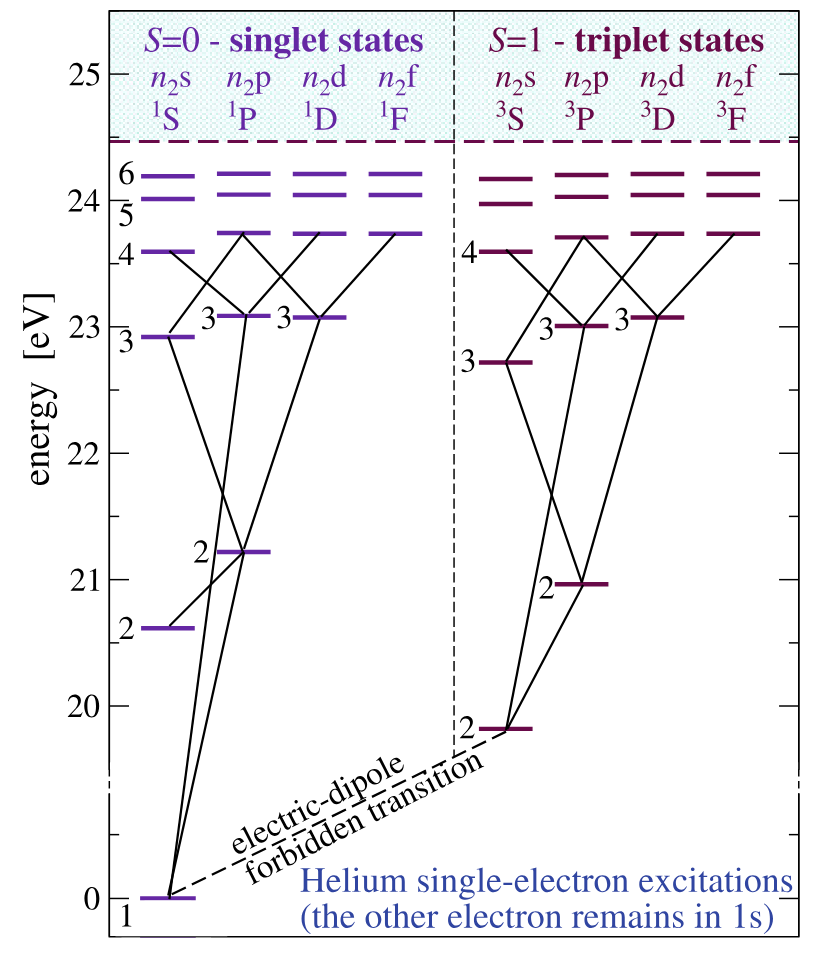
\includegraphics[width = 0.40 \textwidth]{ortho-para-he.png}
	\caption{Energy levels and electric-dipole transitions of atomic $ \ch{He} $.}
	\label{helium}
\end{figure}

\subsection{Elettroni interagenti}
\label{he-inter-electr}

Trattando in maniera perturbativa il potenziale d'interazione $ V_{ee} $, al prim'ordine si ha una correzione all'energia (nelle configurazioni para- o orto-) data da:
\begin{equation*}
	\begin{split}
		\Delta E_{k_1,k_2}^\text{(p,o)}
		& = \braket{\Psi_{k_1,k_2}^\text{(p,o)} | V_{ee} | \Psi_{k_1,k_2}^\text{(p,o)}} = \frac{e^2}{2} \int_{\R^6} \frac{d^3r_1 d^3r_2}{\abs{\ve{r}_1 - \ve{r}_2}}  \abs{\psi_{k_1}(\ve{r}_1) \psi_{k_2}(\ve{r}_2) \pm \psi_{k_1}(\ve{r}_2) \psi_{k_2}(\ve{r}_1)}^2 \\
		& = \frac{e^2}{2} \int_{\R^6} \frac{d^3r_1 d^3r_2}{\abs{\ve{r}_1 - \ve{r}_2}} \left[ \abs{\psi_{k_1}(\ve{r}_1)}^2 \abs{\psi_{k_2}(\ve{r}_2)}^2 + \abs{\psi_{k_1}(\ve{r}_2)}^2 \abs{\psi_{k_2}(\ve{r}_1)}^2 \right] \\
		& \quad \pm \frac{e^2}{2} \int_{\R^6} \frac{d^3r_1 d^3r_2}{\abs{\ve{r}_1 - \ve{r}_2}} \left[ \psi_{k_1}^*(\ve{r}_1) \psi_{k_2}^*(\ve{r}_2) \psi_{k_1}(\ve{r}_2) \psi_{k_2}(\ve{r}_1) + \psi_{k_1}(\ve{r}_1) \psi_{k_2}(\ve{r}_2) \psi_{k_1}^*(\ve{r}_2) \psi_{k_2}^*(\ve{r}_1) \right] \\
		& \equiv E_{k_1,k_2}^\text{(c)} \pm E_{k_1,k_2}^\text{(s)}
	\end{split}
\end{equation*}
dove $ k_i \equiv \{n_i,\ell_i,m_i\} $. $ E^\text{(c)} $ è l'energia dovuta all'interazione Coulombiana, mentre $ E^\text{(s)} $ è dovuta all'interazione di scambio: si dimostra che $ E^\text{(s)} \ge 0 $, dunque la configurazione para- ha un'energia superiore a quella orto- (come si vede in Fig. \ref{helium}). \\
Il fatto che la configurazione orto- sia energeticamente inferiore a quella para- può anche essere dedotto intuitivamente dalla simmetria della funzione d'onda: nel caso orto-, poiché la funzione d'onda spaziale è antisimmetrica, si ha $ \psi(\ve{r},\ve{r}) = 0 $, dunque è molto meno probabile che i due elettroni si trovino vicini rispetto al caso para-. Poiché $ V_{ee} \sim \abs{\ve{r}_1 - \ve{r}_2}^{-1} $, ciò significa che la correzione al prim'ordine dell'energia sarà maggiore nel caso para- rispetto a quello orto-. \\
Gli stati $ (n_1[\ell_1])(n_2[\ell_2]) $ subiscono dunque uno splitting energetico pari a $ 2E^\text{(s)}_{n_1,\ell_1 ; n_2,\ell_2} $ (la dipendenza da $ m $ c'è solo in presenza di campi elettromagnetici esterni che perturbano la simmetria sferica), noto come \textit{splitting da scambio}. Questo splitting è molto importante, poiché sta alla base della \textit{prima regola di Hund}: lo stato energeticamente più basso è sempre quello che massimizza lo spin\footnotemark.

\footnotetext{Ciò nel caso dell'atomo a 2 elettroni non ha alcun effetto sul ground state, poiché esso ha configurazione elettronica $ \text{1s}^2 $, dunque necessariamente $ S = 0 $.}

\section{Atomi a \texorpdfstring{$ N $}{N} elettroni}

L'approccio perturbativo non dà un buon accordo coi dati sperimentali per $ N \ge 3 $: di conseguenza, è necessario adottare un altro metodo. Un'opzione è sfruttare il principio di Ritz (Th. \ref{th:ritz}): supponendo di avere un set di autofunzioni single-particle $ \{\phi_{\alpha_i}(w_i)\}_{i = 1, \dots, N} $ note, è possibile cercare un set di autofunzioni che fungono da base per lo spazio di Hilbert del sistema considerato andando a minimizzare il funzionale energia:
\begin{equation}
	E[\phi_{\alpha_1}, \dots, \phi_{\alpha_N}] = \frac{\braket{\Phi_{\alpha_1, \dots, \alpha_N} | \mathcal{H}_\text{MEA} | \Phi_{\alpha_1, \dots, \alpha_N}}}{\braket{\Phi_{\alpha_1, \dots, \alpha_N} | \Phi_{\alpha_1, \dots, \alpha_N}}}
	\label{eq:en-functional-def}
\end{equation}
dove $ \Phi_{\alpha_1, \dots, \alpha_N} $ è il determinante di Slater delle $ {\phi_{\alpha_i}}_{i = 1, \dots, N} $, le quali sono dette \textit{orbitali atomici}. Essendo $ \mathcal{H}_\text{MEA} = T + V_{ne} + V_{ee} $, si può esplicitare il funzionale come:
\begin{equation}
	\begin{split}
		E[\phi_{\alpha_1}, \dots, \phi_{\alpha_N}]
		& = \sum_{i = 1}^{N} \braket{\alpha_i | \mathcal{H}_0 | \alpha_i} \\
		& \quad + \frac{1}{2} \sum_{i,j = 1}^{N} \int dw\,dw'\, \abs{\phi_{\alpha_i}(w)}^2 v_{ee}(w,w') \abs{\phi_{\alpha_j}(w')}^2 \\
		& \quad - \frac{1}{2} \sum_{i,j = 1}^{N} \int dw\,dw'\, \phi_{\alpha_i}^*(w) \phi_{\alpha_i}(w') v_{ee}(w,w') \phi_{\alpha_j}^*(w') \phi_{\alpha_j}(w)
	\end{split}
	\label{eq:en-functional}
\end{equation}
dove si è assunta l'ortonormalità $ \braket{\alpha_i | \alpha_j} = \delta_{ij} $ e si sono definiti:
\begin{equation}
	\mathcal{H}_0(w) \equiv \left[ -\frac{\hbar^2}{2m_e} \lap_\ve{r} - \frac{Ze^2}{r} \right] \otimes \id_\text{spin}
	\qquad \qquad
	v_{ee}(w,w') \equiv \frac{e^2}{\abs{\ve{r} - \ve{r}'}} \otimes \id_\text{spin}
\end{equation}
Il primo termine del funzionale energia contiene il moto indipendente di ogni elettrone nel potenziale generato dal nucleo, il secondo termine contiene l'interazione Coulombiana tra ciascun elettrone ed la distribuzione di carica media dovuta a tutti gli elettroni, e il terzo termine è un termine di natura non-classica e non-locale dovuto all'antisimmetria per scambio: si noti che il secondo termine contiene anche un'interazione di ciascun elettrone con sé stesso, la quale non ha senso fisico, che viene giustamente cancellata da un addendo nel terzo termine.

\begin{theorem}{Equazione di Hartree-Fock}{eq-hf}
	Il set di autofunzioni $ \{\psi_{\alpha_i}\}_{i = 1, \dots, N} $ che minimizza il funzionale energia soddisfa:
	\begin{equation}
		\mathcal{H}_0(w) \psi_\alpha(w) + V_\text{Ha}(w) \psi_\alpha(w) - \int dw'\, V_\text{Fock}(w,w') \psi_\alpha(w') = E_\alpha \psi_\alpha(w)
	\end{equation}
	dove i potenziali di Hartree e Fock sono definiti come:
	\begin{equation}
		V_\text{Ha}(w) \defeq \int dw'\, \sum_\beta \abs{\phi_\beta(w')}^2 v_{ee}(w,w')
	\end{equation}
	\begin{equation}
		V_\text{Fock}(w,w') \defeq \sum_\beta \phi_\beta^*(w') \phi_\beta(w) v_{ee}(w,w')
	\end{equation}

	\tcblower

	\begin{proof}
		Partendo dall'Eq. \ref{eq:en-functional-def}, si noti che in generale:
		\begin{equation*}
			\frac{\pa E(p)}{\pa p_i} = \frac{\pa}{\pa p_i} \frac{N(p)}{D(p)} = 0
			\quad \Leftrightarrow \quad
			\frac{1}{D(p)} \frac{\pa N(p)}{\pa p_i} - \frac{N(p)}{D^2(p)} \frac{\pa D(p)}{\pa p_i}
			\quad \Leftrightarrow \quad
			\frac{\pa N(p)}{\pa p_i} = E(p) \frac{\pa D(p)}{\pa p_i}
		\end{equation*}
		Applicando la derivata funzionale $ \frac{\delta}{\delta \phi_\alpha^*(w)} $:
		\begin{equation*}
			\frac{\delta}{\delta \phi_\alpha^*(w)} \braket{\Phi_{\alpha_1, \dots, \alpha_N} | \mathcal{H}_\text{MEA} | \Phi_{\alpha_1, \dots, \alpha_N}} = E[\alpha_1, \dots, \alpha_N] \frac{\delta}{\delta \phi_\alpha^*(w)} \braket{\Phi_{\alpha_1, \dots, \alpha_N} | \Phi_{\alpha_1, \dots, \alpha_N}} = E_\alpha \phi_\alpha(w)
		\end{equation*}
		Si calcola la derivata funzionale per ogni termine dell'Eq. \ref{eq:en-functional}:
		\begin{equation*}
			\frac{\delta}{\delta \phi_\alpha^*(w)} \sum_{i = 1}^{N} \braket{\alpha_i | \mathcal{H}_0 | \alpha_i} = \sum_{i = 1}^{N} \delta_{\alpha_i,\alpha} \mathcal{H}_0(w) \phi_{\alpha_i}(w) = \mathcal{H}_0 \phi_\alpha(w)
		\end{equation*}
		\begin{equation*}
			\begin{split}
				\frac{\delta}{\delta \phi_\alpha^*(w)}
				& \frac{1}{2} \sum_{i,j = 1}^{N} \int dw\,dw'\, \abs{\phi_{\alpha_i}(w)}^2 v_{ee}(w,w') \abs{\phi_{\alpha_j}(w')}^2 \\
				& = \frac{1}{2} \sum_{i,j = 1}^{N} \int dw' \left[ \delta_{\alpha_i,\alpha} \phi_{\alpha_i}(w) \abs{\phi_{\alpha_j}(w')}^2 + \abs{\phi_{\alpha_i}(w)}^2 \delta_{\alpha_j,\alpha} \phi_{\alpha_j}(w) \right] v_{ee}(w,w') \\
				& = \sum_{i = 1}^{N} \int dw'\, \abs{\phi_{\alpha_i}(w')}^2 v_{ee}(w,w') \phi_\alpha(w)
			\end{split}
		\end{equation*}
		\begin{equation*}
			\begin{split}
				\frac{\delta}{\delta \phi_\alpha^*(w)}
				& \frac{1}{2} \sum_{i,j = 1}^{N} \int dw\,dw'\, \phi_{\alpha_i}^*(w) \phi_{\alpha_i}(w') v_{ee}(w,w') \phi_{\alpha_j}^*(w') \phi_{\alpha_j}(w) \\
				& = \sum_{i = 1}^{N} \int dw' \phi_{\alpha_i}^*(w') \phi_{\alpha_i}(w) v_{ee}(w,w') \phi_\alpha(w')
			\end{split}
		\end{equation*}
		Rinominando $ \phi_\alpha \equiv \psi_\alpha $ e $ \phi_{\alpha_i} \equiv \phi_\beta $ di ottiene la tesi.
	\end{proof}
\end{theorem}

Si vede che l'equazione HF dipende comunque da un set di autofunzioni $ \{\phi_\beta\} $ ignoto: la strategia di risoluzione consiste nell'assumere che $ \{\phi_\beta\} $ sia un set arbitrario di $ N $ autofunzioni single-particle, risolvere l'equazione HF, scegliere come autofunzioni $ \{\psi_\alpha\} $ le $ N $ soluzioni con autovalore energetico $ E_\alpha $ più basso (\textit{regola dell'Aufbau}) e confrontare i sets $ \{\phi_\beta\} $ e $ \{\psi_\alpha\} $: se essi non variano in maniera apprezzabile (autoconsistenza), si è trovata una soluzione (approssimata) del problema, altrimenti si reitera il processo, assumendo ora $ \{\phi_\beta\} \equiv \{\psi_\alpha\} $. Generalmente si raggiunge l'autoconsistenza in $ 10-100 $ iterazioni. \\
Si noti che non si possono fare assunzioni a priori sul potenziale autoconsistente $ V_\text{HF} $: in  generale, esso non avrà simmetria sferica. Ciò significa che $ E_\alpha $ non avranno l'andamento dell'Eq. \ref{eq:1-e-en}, ma in generale $ E_\alpha = E_{n,\ell} $: ciò spiega l'ordinamento energetico $ n\text{s} < n\text{p} < n\text{d} < \dots $ osservato per gli orbitali atomiche.

\begin{example}{Ground state dell'Argon}{}
	La configurazione elettronica del ground state dell'$ \ch{Ar} $ ($ N = Z = 18 $) è data dalla regola dell'Aufbau e derivata dall'equazione HF: $ \text{1s}^2 \text{2s}^2 \text{2p}^6 \text{3s}^2 \text{3p}^6 $.
\end{example}

\subsection{Atomi idrogenoidi}

Il metodo HF è applicabile anche al caso di un atomo idrogenoide. In tal caso, si considera una generica combinazione di autofunzioni single-particle e si cercano i coefficienti che danno la miglior stima:
\begin{equation*}
	\Psi = \sum_\alpha c_\alpha \phi_\alpha
	\qquad \qquad
	E[\{c_\alpha\}] = \frac{\sum_{\alpha,\beta} c_\alpha^* c_\beta \braket{\phi_\alpha | \mathcal{H} | \phi_\beta}}{\sum_{\alpha,\beta} c_\alpha^* c_\beta \braket{\phi_\alpha | \phi_\beta}} = \frac{\sum_{\alpha,\beta} c_\alpha^* c_\beta \braket{\phi_\alpha | \mathcal{H} | \phi_\beta}}{\sum_\alpha \abs{c_\alpha}^2}
\end{equation*}
assumendo autofunzioni ortonormali $ \braket{\phi_\alpha | \phi_\beta} = \delta_{\alpha\beta} $. Applicando lo stesso ragionamento della dimostrazione del Th. \ref{th:eq-hf}:
\begin{equation*}
	\frac{\pa}{\pa c_k^*} \sum_{\alpha,\beta} c_\alpha^* c_\beta \braket{\phi_\alpha | \mathcal{H} | \phi_\beta} = E[\{c_\alpha\}] \frac{\pa}{\pa c_k^*} \sum_\alpha \abs{c_\alpha}^2
	\quad \Leftrightarrow \quad
	\braket{\phi_k | \mathcal{H} | \Psi} = E_k c_k = E_k \braket{\phi_k | \Psi}
\end{equation*}
L'equazione HF si riduce dunque all'equazione di Schrödinger $ \mathcal{H} \ket{\phi_k} = E_k \ket{\phi_k} $.

\subsection{Tavola periodica}

L'equazione HF permette di predire le configurazioni elettroniche degli elementi della tavola periodiche e le relative proprietà periodiche.

\subsubsection{Configurazioni elettroniche}

Negli elementi fino al $ \ch{Be} $ ($ N \le 4 $) il campo HF gode di simmetria sferica, poiché gli elettroni si dispongono su orbitali $ \text{s} $ perfettamente simmetrici. Per gli elementi successivi, la simmetria sferica è presente soltanto nei gas nobili. \\
Fino all'$ \ch{Ar} $ ($ Z = N = 18 $) gli orbitali vengono riempiti nel consueto ordine, ed infatti la sua configurazione elettronica è $ [\ch{Ar}] = \text{1s}^2 \text{2s}^2 \text{2p}^6 \text{3s}^2 \text{3p}^6 $. Da questo valore di $ Z $, però, la diepndenza di $ E_{n,\ell} $ da $ \ell $ si fa così forte da rendere $ E_\text{3d} > E_\text{4s} $: ciò è sperimentalmente confermato dalla configurazione atomica del potassio $ [\ch{Na}] = [\ch{Ar}] \text{4s}^1 $. Dopo il riempimento della shell $ \text{4s} $ e prima di quello della $ \text{4p} $ avviene il riempimento della $ \text{3d} $: alcune inversioni (es.: $ \ch{Cr} $, $ \ch{Cu} $) mostrano come $ \text{3d} $ e $ \text{4s} $ siano energeticamente molto vicini, così da rendere importanti fenomeni di correlazione elettronica; fenomeni analoghi sono messi in luce anche nel riempimento delle shell $ \text{4d} $, $ \text{4f} $, $ \text{5d} $ e $ \text{5f} $.

\subsubsection{Proprietà periodiche}

L'andamento dell'energia di prima ionizzazione e del raggio atomico degli atomi neutri conferma l'organizzazioni in gruppi della tavola periodica: infatti, atomi con gli stessi elettroni di valenza tendono a comportarsi analogamente.

\begin{figure}
	\centering
	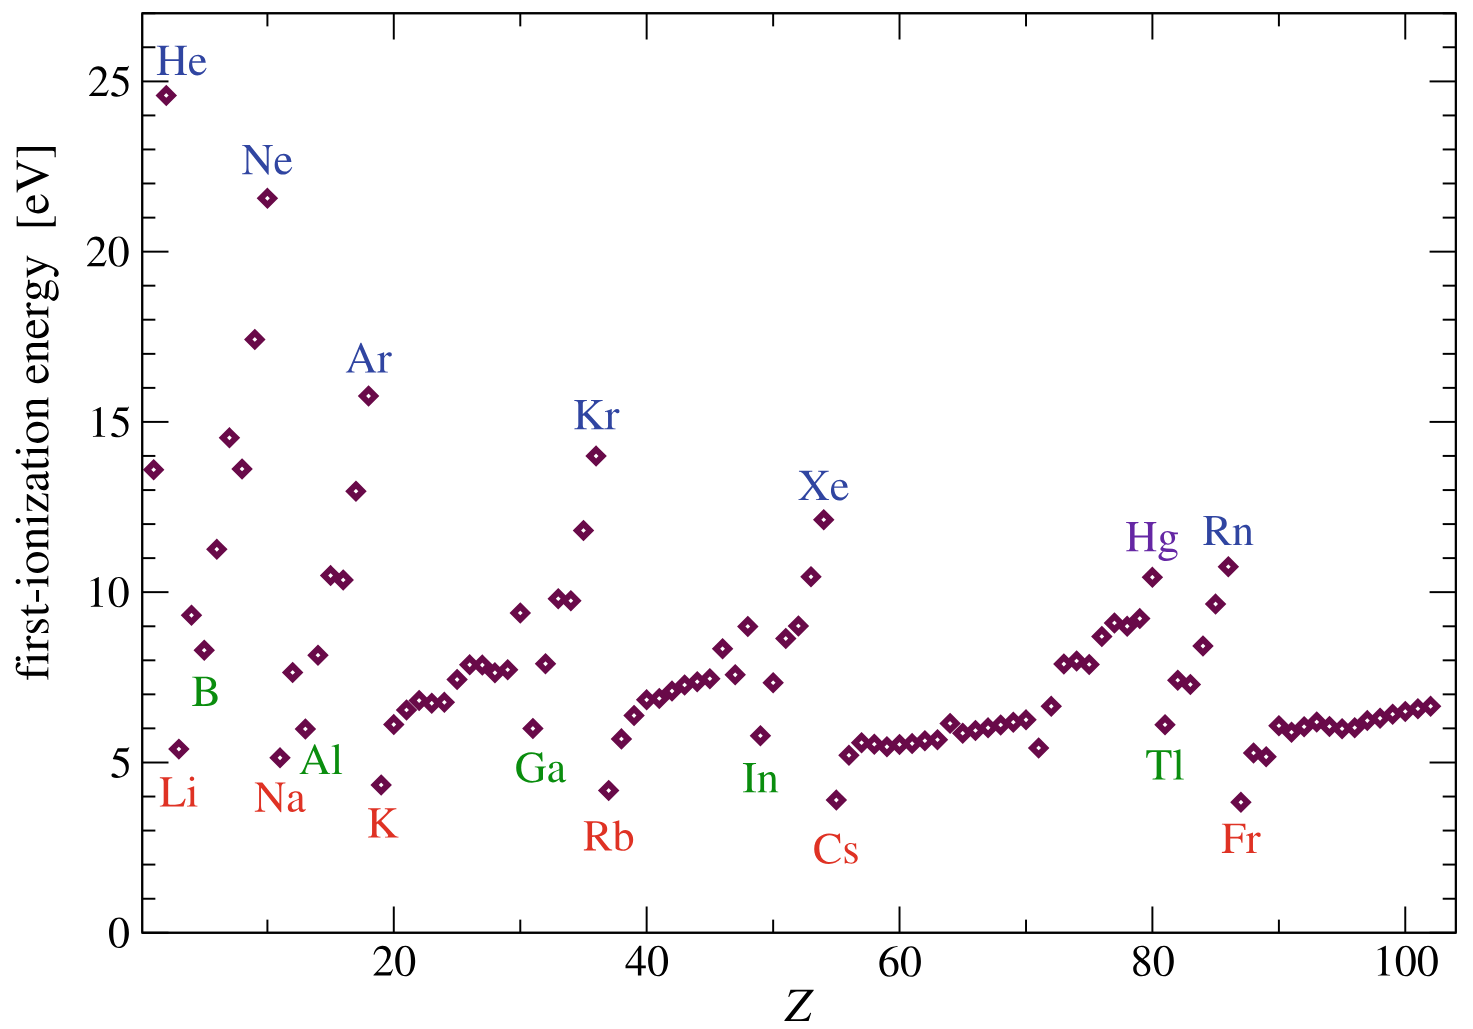
\includegraphics[width = 0.49 \textwidth]{ionization-energy.png}
	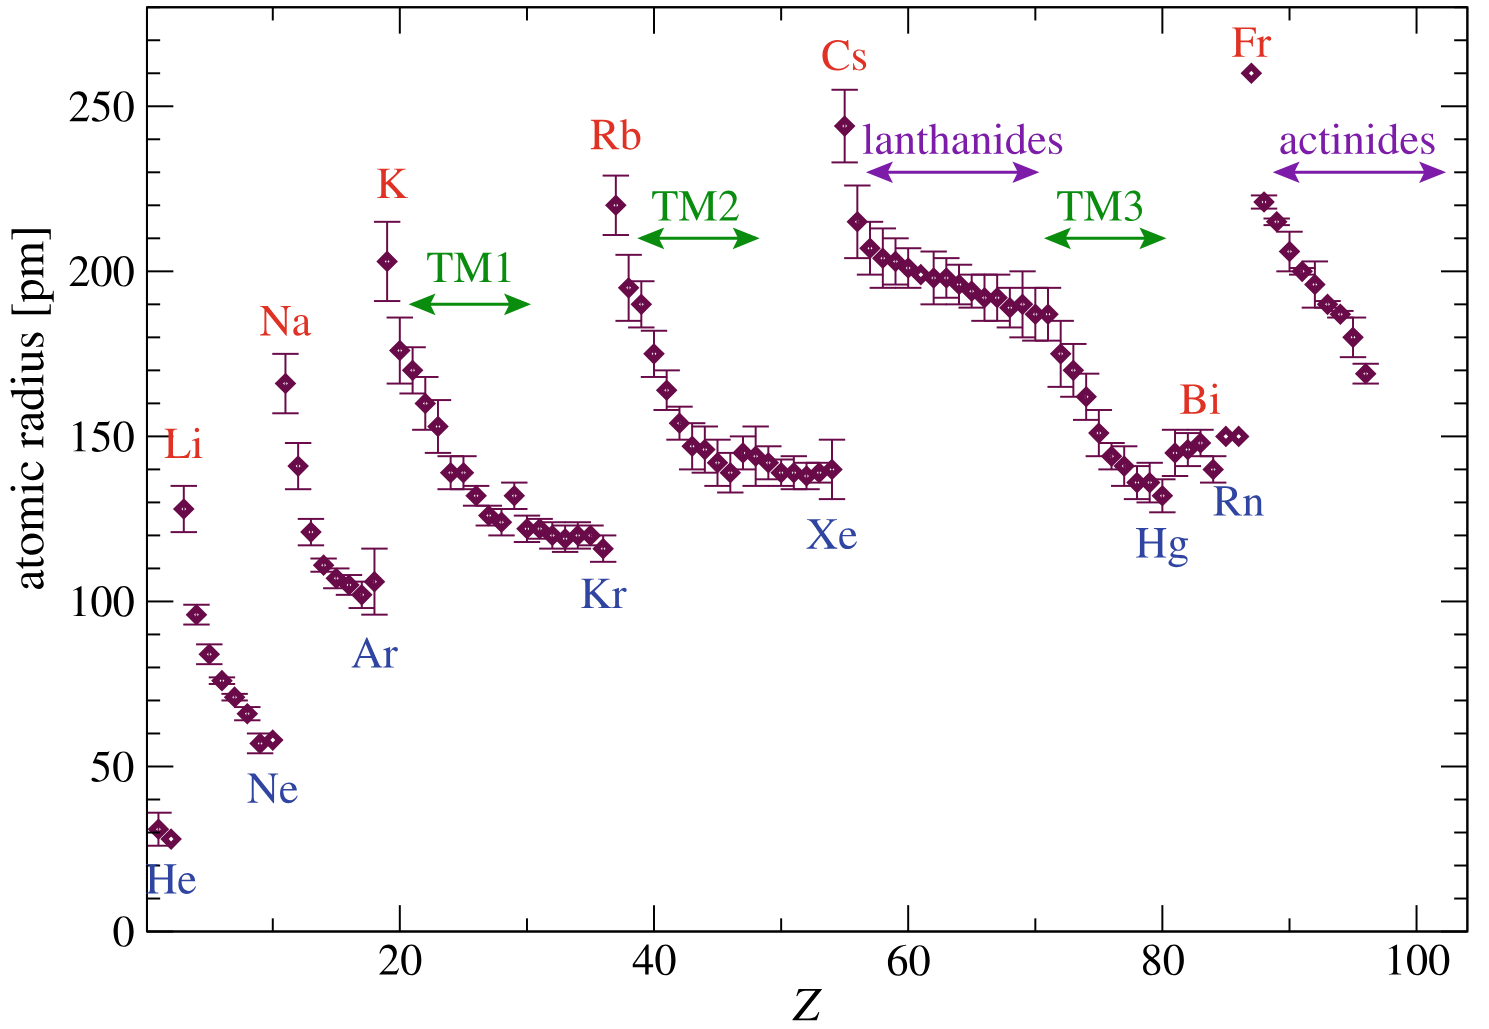
\includegraphics[width = 0.49 \textwidth]{atomic-radius.png}
	\caption{First ionization energy and atomic radius across the periodic table.}
	\label{ion-en-atom-rad}
\end{figure}

Come si può vedere in Fig. \ref{ion-en-atom-rad}, sperimentalmente viene confermato il fatto che i gas nobili hanno shell di valenza complete, poiché presentano energia di prima ionizzazione massima e raggio atomico minimo rispetto agli elementi del loro gruppo. Al contrario, i metalli alcalini hanno un solo elettrone di valenza, per di più molto distante dalle shell interne, come si evince da considerazioni analoghe. \\
Si vede inoltre che gli atomi con shell $ \text{d} $ o $ \text{f} $ incomplete tendono ad avere proprietà (a basse energie) piuttosto uniformi: vengono perciò ragguppati in metalli di transizione ($ \text{3d} $, $ \text{4d} $ e $ \text{5d} $), lantanidi ($ \text{4f} $) ed attinidi ($ \text{5f} $).

\begin{example}{Energia di prima ionizzazione dell'elio}{}
	Se si considera l'$ \ch{He} $, dallo studio della sua energia di ionizzazione si vede come sia necessario considerare l'interazione tra elettroni. Mentre l'energia del catione $ \ch{He}^+ $ è calcolabile usando lo spettro idrogenoide (Eq. \ref{eq:1-e-en}), trovando $ E(\ch{He}^+) = -54\ev $, se si usasse quest'ultimo per calcolare anche l'energia di $ \ch{He} $ si troverebbe $ E(\ch{He}) = 2 E(\ch{He}^+) = - 108\ev $, per un'energia di prima ionizzazione $ E_1(\ch{He}) = 54\ev $ in contrasto col dato sperimentale $ E_1(\ch{He}^+) \simeq 24\ev $. Tenendo conto dell'interazione elettronica, ovvero della correzione in Sec. \ref{he-inter-electr}, si trova $ E(\ch{He}) = -77.8\ev $, ovvero $ E_1(\ch{He}) = 24.2\ev $, dunque in perfetto accordo con le osservazioni.
\end{example}

\subsubsection{Regole di Hund}

Per ottenere la configurazione elettronica del ground state (o degli stati eccitati) di un atomo è necessario svolgere la trattazione HF completa. È però possibile approssimare il risultato utilizzando delle regole semi-empiriche, dette regole di Hund, per stabilire quale, tra tutti gli stati possibili\footnotemark, è il ground state; in ordine di importanza:
\begin{enumerate}
	\item massimizzare lo spin totale $ \bs{S} $;
	\item massimizzare il momento angolare orbitale totale $ \bs{L} $;
	\item per il momento angolare totale $ \bs{J} $, in base al riempimento della shell:
		\begin{itemize}
			\item se è meno di semipiena, minimizzare $ \bs{J} $;
			\item se è più di semipiena, massimizzare $ \bs{J} $.
		\end{itemize}
\end{enumerate}
Queste regole si basano sul minimizzare l'energia del sistema. Per quanto riguarda la prima regola, gli stati atomici a spin più basso hanno energia maggiore poiché, essendo il moto degli elettroni poco correlato, questi tendono a trovarsi in media vicini gli uni agli altri più spesso rispetto agli stati atomici a spin più alto, risultando in una maggiore energia Coulombiana. \\
La seconda regola, invece, deriva dal fatto che, a parità di spin, gli elettroni si evitano più efficientemente quando ruotano in maniera coordinata, ovvero in stati atomici ad alto momento angolare orbitale (a parità di spin, massimizzato dalla prima regola). \\
Infine, massimizzati $ \bs{S} $ ed $ \bs{L} $, rimane da determinare $ \bs{J} $ (poiché $ \bs{S} $ ed $ \bs{L} $ vengono accoppiati dall'interazione spin-orbita): lo stato ad energia minore viene determianto dal segno del coefficiente spin-orbita. Se si considera una shell meno che semipiena, questo sarà naturalmente positivo, ma, se si considera una shell più che semipiena, gli elettroni mancanti possono essere interpretati come particelle di carica opposta, così da avere:
\begin{equation*}
	\mathcal{H}_\text{s-o} = \xi_{n,\ell} \sum_{i = 1}^{n_e} \bs{s}_i \cdot \bs{\ell}_i = \xi_{n,\ell} \underbrace{\sum_{i = 1}^{t} \bs{s}_i \cdot \bs{\ell}_i}_{0} - \xi_{n,\ell} \sum_{i = n_e+1}^{t} \bs{s}_i \cdot \bs{\ell}_i = - \xi_{n,\ell} \sum_{i = n_e + 1}^{t} \bs{s}_i \cdot \bs{\ell}_i
\end{equation*}
Dunque, si vede che nelle shell meno che semipiene va minimizzato $ \bs{J} $, mentre in quelle più che semipiene esso va massimizzato. \\
Si noti che queste regole hanno natura fenomenologica e, sebbene risultino alquanto accurate nel predire i ground states atomici, risultano molto spesso fallaci nella trattazione degli stati eccitati.

\footnotetext{In questo caso, si considerano solo i microstati associati all'ultima shell non completamente riempita: detti $ t $ il numero massimo di elettroni allocabili in tale shell ed $ n_e $ il numero di elettroni da collocarvi, il numero totale di microstati possibili è $ \binom{t}{n_e} $.}

\paragraph{Coupling schemes}

Le regole di Hund si basano sul cosiddetto \textit{Russell-Saunders coupling}, il quale prevede che vengano prima vengano accoppiati i vari $ \bs{s}_i $ a dare $ \bs{S} $ ed i vari $ \bs{\ell}_i $ a dare $ \bs{L} $, e successivamente $ \bs{S} $ ed $ \bs{L} $ vengano accoppiati a dare $ \bs{J} $. Questo coupling scheme risulta efficacie in atomi a basso $ Z $, in cui il potenziale HF (Coulombiano + scambio) è dominante rispetto a quello spin-orbita. \\
Al contrario, per atomi con $ Z \ge 50 $ il potenziale spin-orbita diventa dominante\footnotemark: in questo caso, è necessario prima accoppiare i vari $ \bs{s}_i $ e $ \bs{\ell}_i $, ottenendo i $ \bs{j}_i $ individuali, e poi accoppiare quest'ultimi per ottenere $ \bs{J} $. Questo è noto come \textit{jj coupling}. \\
Mentre la base LS è quasi-diagonale per basso $ Z $ e quella jj lo è per alto $ Z $, a $ Z $ intermedi è necessario diagonalizzare opportunamente sia il termine Coulombiano che quello di spin-orbita.

\footnotetext{Mentre l'energia d'interazione spin-orbita cresce all'aumentare di $ Z $, l'energia d'interazione Coulombiana rimane pressoché costante, risultando addirittura attenuata dal progressivo allontanamento degli elettroni di valenza dal nucleo.}

\section{Spettroscopia}

\subsection{Transizioni di dipolo elettrico}

Nel caso di un sistema ad $ N $ elettroni, l'operatore dipolo elettrico è definito come la somma degli operatori single-particle:
\begin{equation}
	\ve{d} \defeq \sum_{i = 1}^{N} \ve{d}_i = - q_e \sum_{i = 1}^{N} \ve{r}_i
\end{equation}

\begin{proposition}{Transizioni di dipolo elettrico}{}
	Nei sistemi ad $ N $ elettroni, le transizioni di dipolo elettrico sono realizzate da un \textit{singolo elettrone} che transiziona, mentre gli altri rimangono nello stato single-particle iniziale.

	\tcblower

	\begin{proof}
		Nell'approssimazione HF di campo medio:
		\begin{equation*}
			\begin{split}
				& {^\text{(a)}\langle} \beta_1, \dots, \beta_N | \sum_{i = 1}^{N} \ve{d}_i | \alpha_1, \dots, \alpha_N {\rangle^\text{(a)}} = \\
				& \qquad \qquad \qquad = \frac{1}{N!} \sum_{i = 1}^{N} \sum_{\pi,\rho \in S^N} (-1)^{\{\pi\} + \{\rho\}} \braket{\beta_{\pi(1)} | \alpha_{\rho(1)}} \dots \braket{\beta_{\pi(i)} | \ve{d}_i | \alpha_{\rho(i)}} \dots \braket{\beta_{\pi(N)} | \alpha_{\rho(N)}} \\
				& \qquad \qquad \qquad = \frac{1}{N!} \sum_{i = 1}^{N} \sum_{\pi,\rho \in S^N} (-1)^{\{\pi\} + \{\rho\}} \braket{\beta_{\pi(i)} | \ve{d}_i | \alpha_{\rho(i)}} \prod_{j \neq i} \delta_{\beta_{\pi(j)} , \alpha_{\rho(j)}}
			\end{split}
		\end{equation*}
		Si noti che queste $ N - 1 $ delta di Kronecker fissano completamente la permutazione $ \rho \equiv \pi $, dunque:
		\begin{equation*}
			\begin{split}
				{^\text{(a)}\langle} \beta_1, \dots, \beta_N | \sum_{i = 1}^{N} \ve{d}_i | \alpha_1, \dots, \alpha_N {\rangle^\text{(a)}}
				& = \frac{1}{N!} \sum_{i = 1}^{N} \sum_{\pi \in S^N} \braket{\beta_{\pi(i)} | \ve{d}_i | \alpha_{\pi(i)}} \prod_{i \neq j} \delta_{\beta_{\pi(j)} , \alpha_{\pi(j)}} \\
				& = \sum_{i = 1}^{N} \braket{\beta_i | \ve{d}_i | \alpha_i} \prod_{j \neq i} \delta_{\beta_j , \alpha_j}
			\end{split}
		\end{equation*}
		Ciò equivale alla tesi.
	\end{proof}
\end{proposition}

Dato che le transizioni di dipolo-elettrico di un sistema ad $ N $ elettroni si riducono a quelle single-particle, si ha che le transizioni ammesse sono quelle in cui la configurazione elettronica dell'atomo cambia per un solo elettrone, tale per cui $ \Delta \ell_i = \pm 1 $ (più le altre condizioni in Eq. \ref{eq:1-e-el-dip-tr-m}-\ref{eq:1-e-el-dip-tr-spin}).

\begin{example}{Transizioni di dipolo elettrico del berillio}{}
	La configurazione elettronica del ground state del berillio è $ [\ch{Be}] = \text{1s}^2 \text{2s}^2 $. Possibili transizioni di dipolo elettrico ammesse sono $ \text{1s}^2 \text{2s}^2 \rightarrow \text{1s}^2 \text{2s}^1 \text{2p}^1 $ o $ \text{1s}^1 \text{2s}^2 \text{2p}^1 \rightarrow \text{1s}^1 \text{2s}^2 \text{4d}^1 $; transizioni proibite sono invece $ \text{1s}^2 \text{2s}^2 \rightarrow \text{1s}^2 \text{2s}^1 \text{3d}^1 $ o $ \text{1s}^2 \text{2s}^2 \rightarrow \text{1s}^1 \text{2s}^1 \text{2p}^1 \text{3p}^1 $.
\end{example}

\subsection{Eccitazioni di core}

Secondo la teoria HF, gli stati di core (single-particle), ovvero tutti gli elettroni non di valenza, subiscono una schermatura del potenziale del nucleo trascurabile, dunque la loro energia è molto negativa ($ \propto - Z^2 $): ciò è confermato dal fatto che, se per esempio si considera un eccitazione del $ \ch{Na} $ del tipo $ \text{1s}^2 \text{2s}^2 \text{2p}^6 \text{3s}^1 \rightarrow \text{1s}^1 \text{2s}^2 \text{2p}^6 \text{3s}^2 $, sono necessarie energie dell'ordine $ \sim 1\kev $ per eccitare gli stati di core al primo stato eccitato disponibile (a causa del principio d'esclusione). \\
Ne consegue che, data la dipendenza del decay rate da $ E_\text{if}^3 $, le eccitazioni di core presentano delle linee spettrali estremamente allargate, oltre $ \hbar \gamma \sim 1\ev $. Inoltre, dall'Eq. \ref{eq:electric-dipole-decay-rate}, si vede che $ \gamma \sim Z^4 $.

\begin{figure}
	\centering
	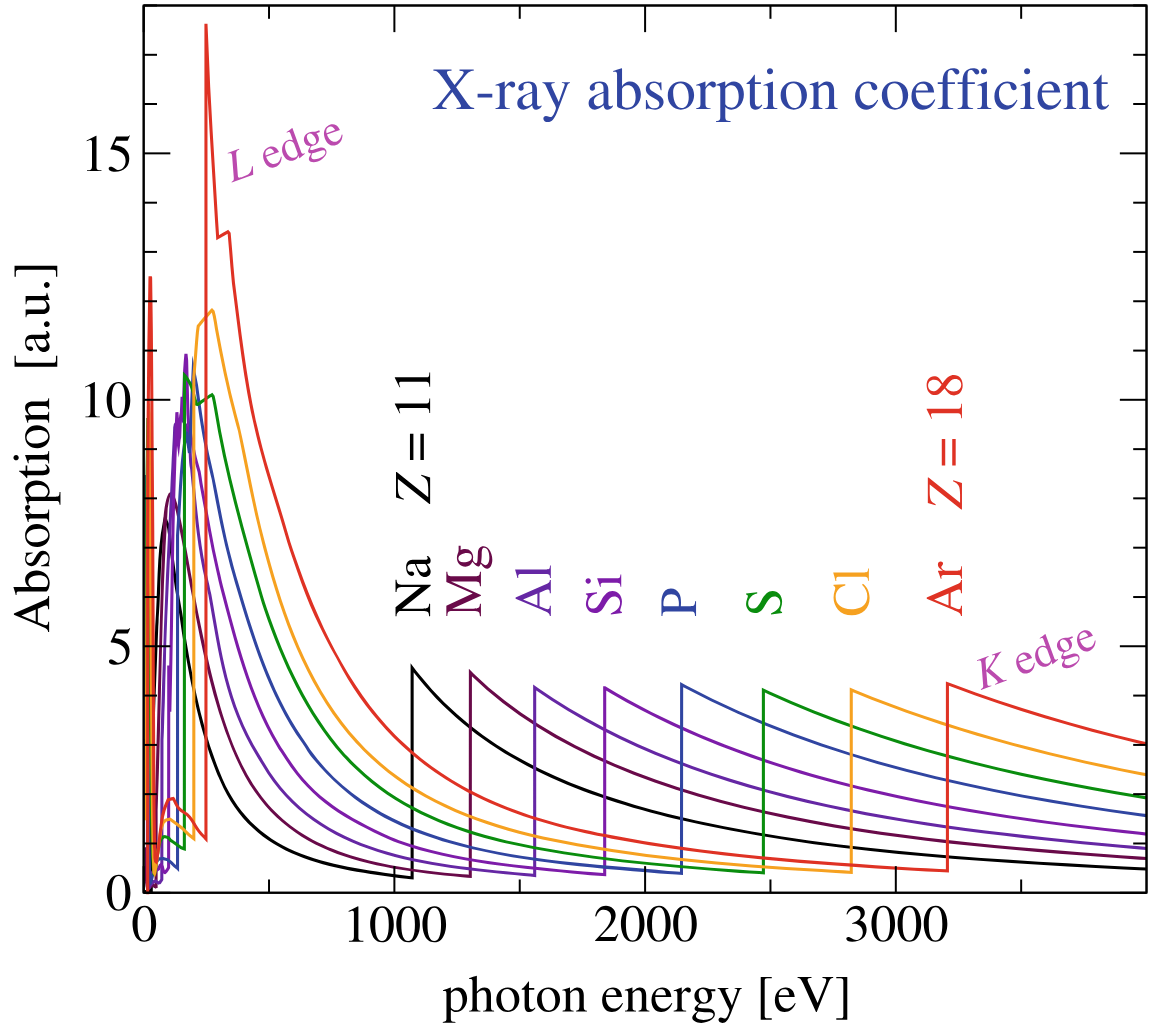
\includegraphics[width = 0.45 \textwidth]{core-exc-x-rays.png}
	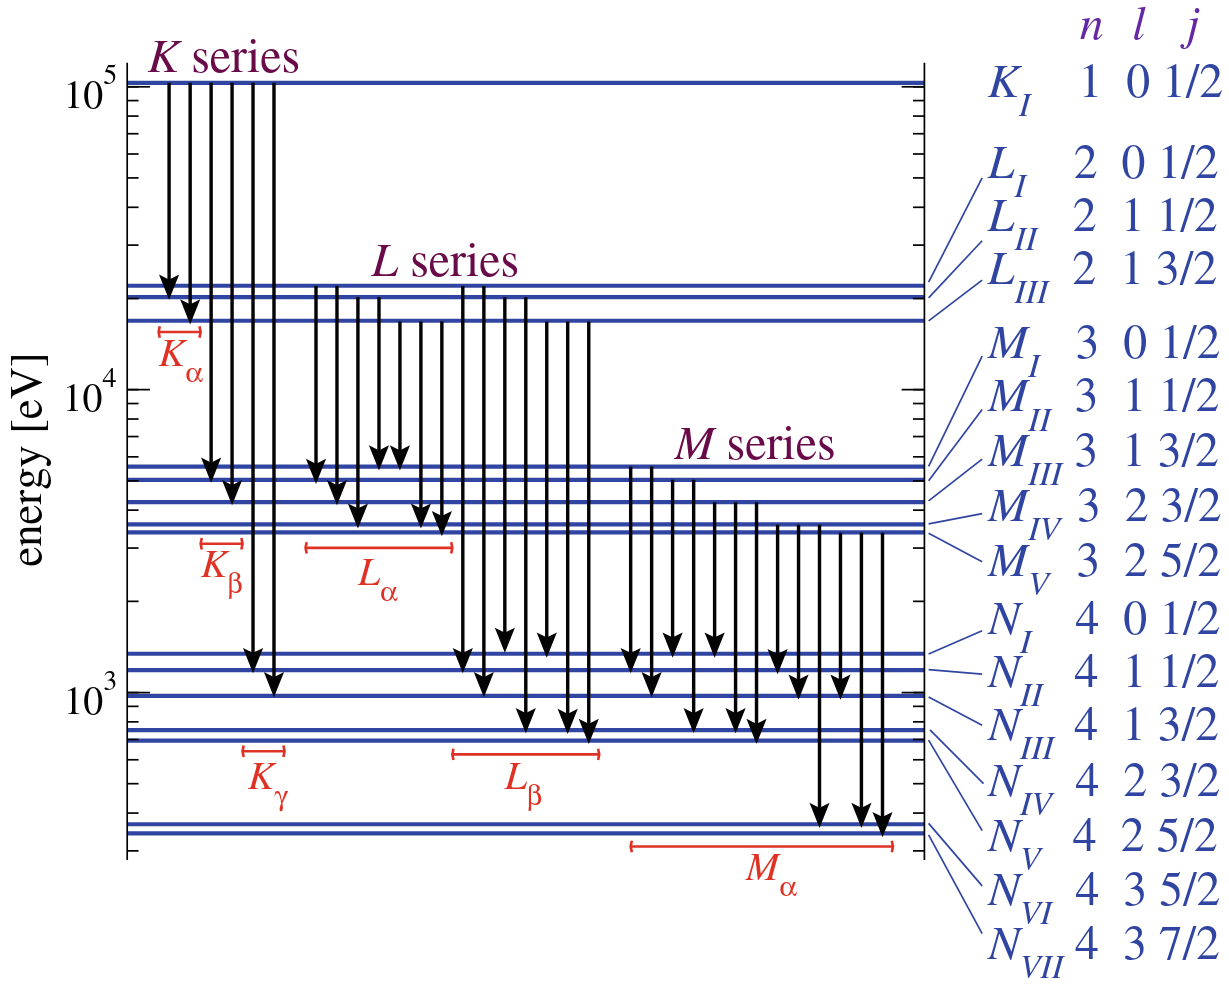
\includegraphics[width = 0.45 \textwidth]{core-exc-spectr.png}
	\caption{Observed X-ray absorption for third-period elements and observed core-level structure of $ \ch{U} $.}
	\label{core-exc}
\end{figure}

Le eccitazioni di core sono molto studiate a livello sperimentale: as esempio, i dati relativi all'assorbimento di raggi X (Fig. \ref{core-exc}) mostrano una certa regolarità per $ E_\gamma > 50\ev $, con un andamento sistematico rispetto a $ Z $. In particolare, si vede che negli spettri d'assorbimento di raggi X i picchi hanno una forma asimmetrica: per quanto riguarda l'estremità energeticamente inferiore, non può avvenire alcun assorbimento, in quanto l'energia non sarebbe sufficiente ad eccitare l'elettrone di core al primo stato eccitato libero (e, per il principio d'esclusione, esso non può essere eccitato a nessuno stato al di sotto di questo); superata la soglia d'assorbimento, invece, l'elettrone può essere eccitato a vari stati non-occupati, sia legati che non, risultando in uno spettro d'assorbimento continuo. \\
Si noti, inoltre, che all'aumentare dell'energia del fotone assorbito aumenta anche l'energia cinetica dell'elettrone ($ K_e = E_\gamma - E_\text{exc} $): conseguentemente, lo stato eccitato finale diventa progressivamente più ortogonale a quello iniziale. Ciò determina una rapida diminuzione di $ \gamma_\text{if} \propto \braket{\text{i} | \ve{d} | \text{f}} $, ovvero un rallentamento del decadimento. Per lo stesso motivo, inoltre, si capisce perché l'assorbimento di raggi X genera eccitazioni di core: se il fotone fosse assorbito da un elettrone di valenza, il quale è debolmente legato, la sua energia cinetica sarebbe molto alta, rendendo lo stato eccitato molto ortogonale rispetto a quello iniziale e rendendo $ \gamma $ trascurabile.

\subsubsection{Legge di Moseley}

Per quanto riguarda le transizioni tra stati di core, si adotta la seguente notazione: un \textit{hole} (elettrone mancante) in una shell $ n = 1,2,3,4,\dots$ è indicato da $ K,L,M,N,\dots $, mentre il numero di salti di shell è indicato da $ \alpha,\beta,\gamma,\dots$.

\begin{example}{Transizioni di core}{}
	Una transizione del tipo $ \text{1s}^1 \text{2s}^2 \text{2p}^6 \dots \rightarrow \text{1s}^2 \text{2s}^2 \text{2p}^5 \dots $ è indicata come $ K_\alpha \equiv K \rightarrow L $. Una transizione del tipo $ \text{1s}^2 \text{2s}^2 \text{2p}^5 \text{3s}^2 \text{3p}^6 \text{4s}^2 \dots \rightarrow \text{1s}^2 \text{2s}^2 \text{2p}^6 \text{3s}^2 \text{3p}^6 \text{4s}^1 \dots $ è $ L_\beta \equiv L \rightarrow N $.
\end{example}

Per quanto riguarda le linee spettrali $ K_\alpha $, dai dati sperimentali si evince una legge fenomenologica, detta \textit{legge di Moseley}:
\begin{equation}
	\frac{1}{\lambda_{K_\alpha}} \approx C \left( Z - a \right)^2
\end{equation}
dove $ C \approx \frac{3}{8} \frac{E_\text{Ha}}{2\pi \hbar c} \simeq 8.25 \cdot 10^6 \,\text{m}^{-1} $ ed $ a $ è il \textit{parametro di screening}. Quest'ultimo tiene conto dello screening che la carica nucleare subisce a causa degli elettroni di core (vedere Fig. \ref{screening}): non c'è una definizione ben precisa di $ a $, in quanto è un parametro fenomenologico, ma un buon accordo coi dati sperimentali è dato dal numero di elettroni nelle shell più interne a quelle considerate, includendo anche quella in esame (dunque $ (n,a) = (1,2) , (2,10), (3,28), \dots $).

\begin{figure}
	\centering
	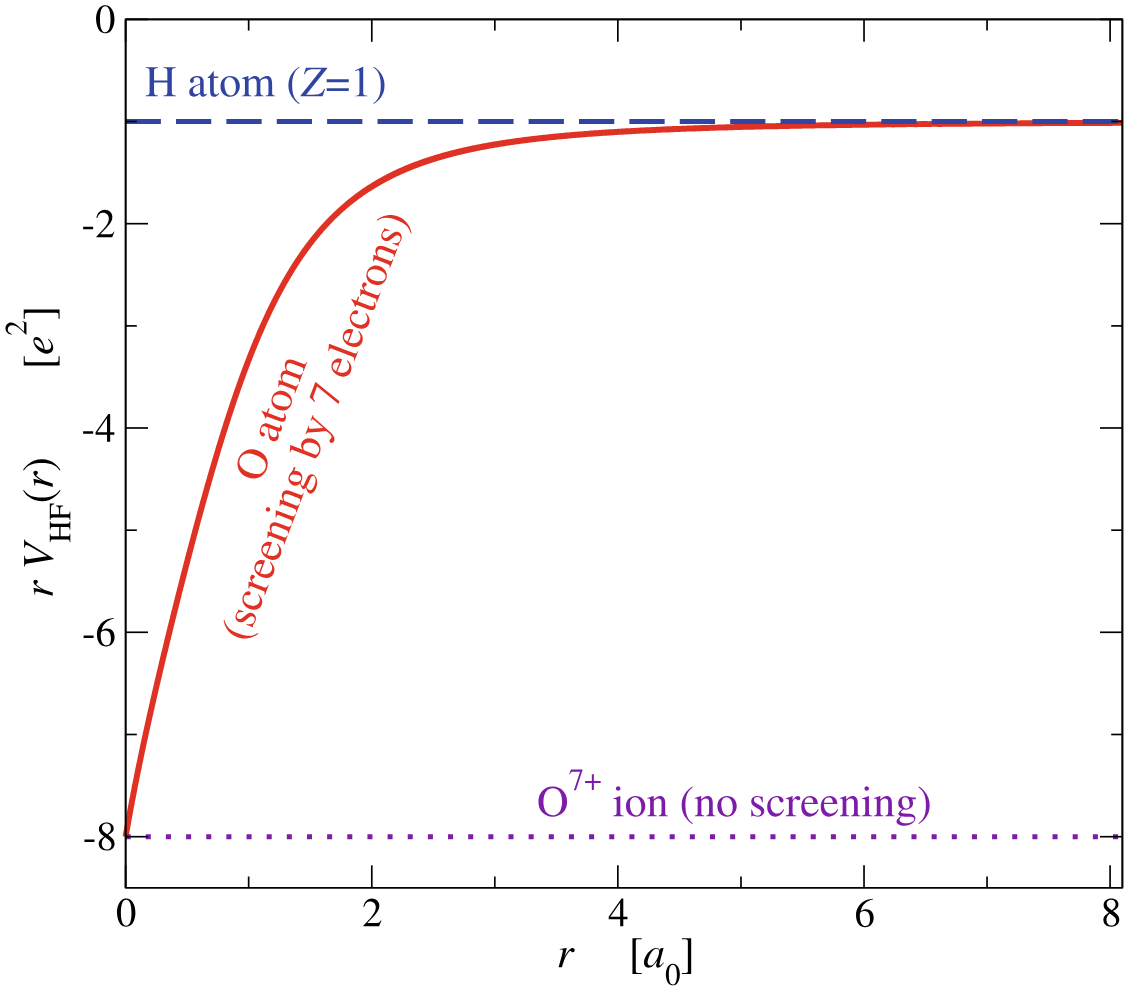
\includegraphics[width = 0.50 \textwidth]{screening.png}
	\caption{HF effective potential for atomic $ \ch{O} $ ($ N = Z = 8 $).}
	\label{screening}
\end{figure}

\subsection{Campo magnetico esterno}

Quando viene applicato un campo magnetico ad un MAE, si osserva un comportamento diverso in base alla presenza o meno di un momento magnetico. \\
Se si considera un atomo con $ J = 0 $, esso non ha alcun momento magnetico permanente: il campo esterno induce un piccolo momento magnetico $ \mu \sim \mu_\text{B} \frac{\mu_\text{B} B}{\Delta} $, dove $ \Delta $ è la differenza energetica tra il ground state ed il primo stato eccitato con $ J \neq 0 $, ma questi effetti sono trascurabili. \\
Al contrario, atomi con $ J \neq 0 $ hanno un momento magnetico permanente:
\begin{equation}
	\bs{\mu} = - g_J \mu_\text{B} \bs{J}
\end{equation}
dove $ g_J $ è il fattore di Landé (Eq. \ref{eq:lande-g-factor} con $ S,L,J $, nel LS coupling). Questo momento mangetico è rilevante nel limite Zeeman di campo esterno debole, che nella pratica è quello più importante in quanto difficilmente in laboratorio di riescono a produrre campi magnetici tali da dominare sull'interazione spin-orbita. \\
Per quanto riguarda lo splitting delle linee spettrali, si distingue tra \textit{regular Zeeman splitting}, nel caso in cui esse vengano splittate regolamente in $ 2J + 1 $ linee spettrali (quando i fattori di Landé dello stato iniziale e finale sono uguali), e \textit{anomalous Zeeman splitting}, nel caso in cui lo splitting pattern sia più complesso (quando i fattori di Landé dello stato iniziale e finale sono diversi). \\
Un'importante strumento sperimentale per studiare la degenerazione dei ground states dei MAE è l'apparato di Stern-Gerlach, nel quale gli atomi vengono deflessi (Eq. \ref{eq:stern-gerlach}) secondo:
\begin{equation*}
	F_z = \mu_z \frac{\pa B_z}{\pa z} = - g_J \mu_\text{B} M_J \frac{\pa B_z}{\pa z}
\end{equation*}
Il numero di sotto-fasci in cui viene splittato il fascio iniziale dà dunque una misura diretta dei possibili valori di $ M_J $, ovvero della degenerazione $ 2J + 1 $ del ground state.












\end{document}
